% % bare_jrnl_compsoc.tex
%% V1.4b
%% 2015/08/26
%% by Michael Shell
%% See:
%% http://www.michaelshell.org/
%% for current contact information.
%%
%% This is a skeleton file demonstrating the use of IEEEtran.cls
%% (requires IEEEtran.cls version 1.8b or later) with an IEEE
%% Computer Society journal paper.
%%
%% Support sites:
%% http://www.michaelshell.org/tex/ieeetran/
%% http://www.ctan.org/pkg/ieeetran
%% and
%% http://www.ieee.org/

%%*************************************************************************
%% Legal Notice:
%% This code is offered as-is without any warranty either expressed or
%% implied; without even the implied warranty of MERCHANTABILITY or
%% FITNESS FOR A PARTICULAR PURPOSE! 
%% User assumes all risk.
%% In no event shall the IEEE or any contributor to this code be liable for
%% any damages or losses, including, but not limited to, incidental,
%% consequential, or any other damages, resulting from the use or misuse
%% of any information contained here.
%%
%% All comments are the opinions of their respective authors and are not
%% necessarily endorsed by the IEEE.
%%
%% This work is distributed under the LaTeX Project Public License (LPPL)
%% ( http://www.latex-project.org/ ) version 1.3, and may be freely used,
%% distributed and modified. A copy of the LPPL, version 1.3, is included
%% in the base LaTeX documentation of all distributions of LaTeX released
%% 2003/12/01 or later.
%% Retain all contribution notices and credits.
%% ** Modified files should be clearly indicated as such, including  **
%% ** renaming them and changing author support contact information. **
%%*************************************************************************


% *** Authors should verify (and, if needed, correct) their LaTeX system  ***
% *** with the testflow diagnostic prior to trusting their LaTeX platform ***
% *** with production work. The IEEE's font choices and paper sizes can   ***
% *** trigger bugs that do not appear when using other class files.       ***                          ***
% The testflow support page is at:
% http://www.michaelshell.org/tex/testflow/


\documentclass[10pt,journal,compsoc]{IEEEtran}
%
% If IEEEtran.cls has not been installed into the LaTeX system files,
% manually specify the path to it like:
% \documentclass[10pt,journal,compsoc]{../sty/IEEEtran}





% Some very useful LaTeX packages include:
% (uncomment the ones you want to load)


% *** MISC UTILITY PACKAGES ***
%
%\usepackage{ifpdf}
% Heiko Oberdiek's ifpdf.sty is very useful if you need conditional
% compilation based on whether the output is pdf or dvi.
% usage:
% \ifpdf
%   % pdf code
% \else
%   % dvi code
% \fi
% The latest version of ifpdf.sty can be obtained from:
% http://www.ctan.org/pkg/ifpdf
% Also, note that IEEEtran.cls V1.7 and later provides a builtin
% \ifCLASSINFOpdf conditional that works the same way.
% When switching from latex to pdflatex and vice-versa, the compiler may
% have to be run twice to clear warning/error messages.






% *** CITATION PACKAGES ***
%
\ifCLASSOPTIONcompsoc
  % IEEE Computer Society needs nocompress option
  % requires cite.sty v4.0 or later (November 2003)
  \usepackage[nocompress]{cite}
\else
  % normal IEEE
  \usepackage{cite}
\fi

\usepackage{xcolor}
\usepackage{algorithm}
\usepackage{algorithmic}
\usepackage{listings}
\usepackage{multicol}
\usepackage{subcaption}
\usepackage{wrapfig}


\usepackage[skins,theorems]{tcolorbox}
\tcbset{highlight math style={enhanced,
  colframe=red,colback=white,arc=0pt,boxrule=1pt}}

% define custom commands for creating references
% for tables, figures, equations and such
\newcommand{\eref}[1]{\eqref{#1}}        % cite equation
\newcommand{\fref}[1]{Figure~\ref{#1}}   % cite figure
\newcommand{\cref}[1]{Chapter~\ref{#1}}  % cite chapter
\newcommand{\sref}[1]{Section~\ref{#1}}  % cite section/sub(sub)section
\newcommand{\aref}[1]{Appendix~\ref{#1}} % cite appendix
\newcommand{\tref}[1]{Table~\ref{#1}}    % cite table
\newcommand{\alphaz}{\textsc{\texttt{AlphaZ}}}
\newcommand{\alfa}{\textsc{\texttt{Alpha}}}
\newcommand*{\colorboxed}{}
\def\colorboxed#1#{%
  \colorboxedAux{#1}%
}
\newcommand*{\colorboxedAux}[3]{%
  % #1: optional argument for color model
  % #2: color specification
  % #3: formula
  \begingroup
    \colorlet{cb@saved}{.}%
    \color#1{#2}%
    \boxed{%
      \color{cb@saved}%
      #3%
    }%
  \endgroup
}

\definecolor{deepskyblue}{rgb}{0.0, 0.75, 1.0}
\definecolor{green(ryb)}{rgb}{0.4, 0.69, 0.2}
\definecolor{orange(webcolor)}{rgb}{1.0, 0.65, 0.0}

\usepackage{xcolor}


\newsavebox\MBox
\newcommand\Cline[2][red]{{\sbox\MBox{$#2$}%
  \rlap{\usebox\MBox}\color{#1}\rule[-1.2\dp\MBox]{\wd\MBox}{0.5pt}}}

% cite.sty was written by Donald Arseneau
% V1.6 and later of IEEEtran pre-defines the format of the cite.sty package
% \cite{} output to follow that of the IEEE. Loading the cite package will
% result in citation numbers being automatically sorted and properly
% "compressed/ranged". e.g., [1], [9], [2], [7], [5], [6] without using
% cite.sty will become [1], [2], [5]--[7], [9] using cite.sty. cite.sty's
% \cite will automatically add leading space, if needed. Use cite.sty's
% noadjust option (cite.sty V3.8 and later) if you want to turn this off
% such as if a citation ever needs to be enclosed in parenthesis.
% cite.sty is already installed on most LaTeX systems. Be sure and use
% version 5.0 (2009-03-20) and later if using hyperref.sty.
% The latest version can be obtained at:
% http://www.ctan.org/pkg/cite
% The documentation is contained in the cite.sty file itself.
%
% Note that some packages require special options to format as the Computer
% Society requires. In particular, Computer Society  papers do not use
% compressed citation ranges as is done in typical IEEE papers
% (e.g., [1]-[4]). Instead, they list every citation separately in order
% (e.g., [1], [2], [3], [4]). To get the latter we need to load the cite
% package with the nocompress option which is supported by cite.sty v4.0
% and later. Note also the use of a CLASSOPTION conditional provided by
% IEEEtran.cls V1.7 and later.

% *** GRAPHICS RELATED PACKAGES ***
%
\ifCLASSINFOpdf
  % \usepackage[pdftex]{graphicx}
  % declare the path(s) where your graphic files are
  % \graphicspath{{../pdf/}{../jpeg/}}
  % and their extensions so you won't have to specify these with
  % every instance of \includegraphics
  % \DeclareGraphicsExtensions{.pdf,.jpeg,.png}
\else
  % or other class option (dvipsone, dvipdf, if not using dvips). graphicx
  % will default to the driver specified in the system graphics.cfg if no
  % driver is specified.
  % \usepackage[dvips]{graphicx}
  % declare the path(s) where your graphic files are
  % \graphicspath{{../eps/}}
  % and their extensions so you won't have to specify these with
  % every instance of \includegraphics
  % \DeclareGraphicsExtensions{.eps}
\fi
% graphicx was written by David Carlisle and Sebastian Rahtz. It is
% required if you want graphics, photos, etc. graphicx.sty is already
% installed on most LaTeX systems. The latest version and documentation
% can be obtained at: 
% http://www.ctan.org/pkg/graphicx
% Another good source of documentation is "Using Imported Graphics in
% LaTeX2e" by Keith Reckdahl which can be found at:
% http://www.ctan.org/pkg/epslatex
%
% latex, and pdflatex in dvi mode, support graphics in encapsulated
% postscript (.eps) format. pdflatex in pdf mode supports graphics
% in .pdf, .jpeg, .png and .mps (metapost) formats. Users should ensure
% that all non-photo figures use a vector format (.eps, .pdf, .mps) and
% not a bitmapped formats (.jpeg, .png). The IEEE frowns on bitmapped formats
% which can result in "jaggedy"/blurry rendering of lines and letters as
% well as large increases in file sizes.
%
% You can find documentation about the pdfTeX application at:
% http://www.tug.org/applications/pdftex






% *** MATH PACKAGES ***
%
%\usepackage{amsmath}
% A popular package from the American Mathematical Society that provides
% many useful and powerful commands for dealing with mathematics.
%
% Note that the amsmath package sets \interdisplaylinepenalty to 10000
% thus preventing page breaks from occurring within multiline equations. Use:
%\interdisplaylinepenalty=2500
% after loading amsmath to restore such page breaks as IEEEtran.cls normally
% does. amsmath.sty is already installed on most LaTeX systems. The latest
% version and documentation can be obtained at:
% http://www.ctan.org/pkg/amsmath





% *** SPECIALIZED LIST PACKAGES ***
%
%\usepackage{algorithmic}
% algorithmic.sty was written by Peter Williams and Rogerio Brito.
% This package provides an algorithmic environment fo describing algorithms.
% You can use the algorithmic environment in-text or within a figure
% environment to provide for a floating algorithm. Do NOT use the algorithm
% floating environment provided by algorithm.sty (by the same authors) or
% algorithm2e.sty (by Christophe Fiorio) as the IEEE does not use dedicated
% algorithm float types and packages that provide these will not provide
% correct IEEE style captions. The latest version and documentation of
% algorithmic.sty can be obtained at:
% http://www.ctan.org/pkg/algorithms
% Also of interest may be the (relatively newer and more customizable)
% algorithmicx.sty package by Szasz Janos:
% http://www.ctan.org/pkg/algorithmicx




% *** ALIGNMENT PACKAGES ***
%
%\usepackage{array}
% Frank Mittelbach's and David Carlisle's array.sty patches and improves
% the standard LaTeX2e array and tabular environments to provide better
% appearance and additional user controls. As the default LaTeX2e table
% generation code is lacking to the point of almost being broken with
% respect to the quality of the end results, all users are strongly
% advised to use an enhanced (at the very least that provided by array.sty)
% set of table tools. array.sty is already installed on most systems. The
% latest version and documentation can be obtained at:
% http://www.ctan.org/pkg/array


% IEEEtran contains the IEEEeqnarray family of commands that can be used to
% generate multiline equations as well as matrices, tables, etc., of high
% quality.




% *** SUBFIGURE PACKAGES ***
%\ifCLASSOPTIONcompsoc
%  \usepackage[caption=false,font=footnotesize,labelfont=sf,textfont=sf]{subfig}
%\else
%  \usepackage[caption=false,font=footnotesize]{subfig}
%\fi
% subfig.sty, written by Steven Douglas Cochran, is the modern replacement
% for subfigure.sty, the latter of which is no longer maintained and is
% incompatible with some LaTeX packages including fixltx2e. However,
% subfig.sty requires and automatically loads Axel Sommerfeldt's caption.sty
% which will override IEEEtran.cls' handling of captions and this will result
% in non-IEEE style figure/table captions. To prevent this problem, be sure
% and invoke subfig.sty's "caption=false" package option (available since
% subfig.sty version 1.3, 2005/06/28) as this is will preserve IEEEtran.cls
% handling of captions.
% Note that the Computer Society format requires a sans serif font rather
% than the serif font used in traditional IEEE formatting and thus the need
% to invoke different subfig.sty package options depending on whether
% compsoc mode has been enabled.
%
% The latest version and documentation of subfig.sty can be obtained at:
% http://www.ctan.org/pkg/subfig




% *** FLOAT PACKAGES ***
%
%\usepackage{fixltx2e}
% fixltx2e, the successor to the earlier fix2col.sty, was written by
% Frank Mittelbach and David Carlisle. This package corrects a few problems
% in the LaTeX2e kernel, the most notable of which is that in current
% LaTeX2e releases, the ordering of single and double column floats is not
% guaranteed to be preserved. Thus, an unpatched LaTeX2e can allow a
% single column figure to be placed prior to an earlier double column
% figure.
% Be aware that LaTeX2e kernels dated 2015 and later have fixltx2e.sty's
% corrections already built into the system in which case a warning will
% be issued if an attempt is made to load fixltx2e.sty as it is no longer
% needed.
% The latest version and documentation can be found at:
% http://www.ctan.org/pkg/fixltx2e


%\usepackage{stfloats}
% stfloats.sty was written by Sigitas Tolusis. This package gives LaTeX2e
% the ability to do double column floats at the bottom of the page as well
% as the top. (e.g., "\begin{figure*}[!b]" is not normally possible in
% LaTeX2e). It also provides a command:
%\fnbelowfloat
% to enable the placement of footnotes below bottom floats (the standard
% LaTeX2e kernel puts them above bottom floats). This is an invasive package
% which rewrites many portions of the LaTeX2e float routines. It may not work
% with other packages that modify the LaTeX2e float routines. The latest
% version and documentation can be obtained at:
% http://www.ctan.org/pkg/stfloats
% Do not use the stfloats baselinefloat ability as the IEEE does not allow
% \baselineskip to stretch. Authors submitting work to the IEEE should note
% that the IEEE rarely uses double column equations and that authors should try
% to avoid such use. Do not be tempted to use the cuted.sty or midfloat.sty
% packages (also by Sigitas Tolusis) as the IEEE does not format its papers in
% such ways.
% Do not attempt to use stfloats with fixltx2e as they are incompatible.
% Instead, use Morten Hogholm'a dblfloatfix which combines the features
% of both fixltx2e and stfloats:
%
% \usepackage{dblfloatfix}
% The latest version can be found at:
% http://www.ctan.org/pkg/dblfloatfix




%\ifCLASSOPTIONcaptionsoff
%  \usepackage[nomarkers]{endfloat}
% \let\MYoriglatexcaption\caption
% \renewcommand{\caption}[2][\relax]{\MYoriglatexcaption[#2]{#2}}
%\fi
% endfloat.sty was written by James Darrell McCauley, Jeff Goldberg and 
% Axel Sommerfeldt. This package may be useful when used in conjunction with 
% IEEEtran.cls'  captionsoff option. Some IEEE journals/societies require that
% submissions have lists of figures/tables at the end of the paper and that
% figures/tables without any captions are placed on a page by themselves at
% the end of the document. If needed, the draftcls IEEEtran class option or
% \CLASSINPUTbaselinestretch interface can be used to increase the line
% spacing as well. Be sure and use the nomarkers option of endfloat to
% prevent endfloat from "marking" where the figures would have been placed
% in the text. The two hack lines of code above are a slight modification of
% that suggested by in the endfloat docs (section 8.4.1) to ensure that
% the full captions always appear in the list of figures/tables - even if
% the user used the short optional argument of \caption[]{}.
% IEEE papers do not typically make use of \caption[]'s optional argument,
% so this should not be an issue. A similar trick can be used to disable
% captions of packages such as subfig.sty that lack options to turn off
% the subcaptions:
% For subfig.sty:
% \let\MYorigsubfloat\subfloat
% \renewcommand{\subfloat}[2][\relax]{\MYorigsubfloat[]{#2}}
% However, the above trick will not work if both optional arguments of
% the \subfloat command are used. Furthermore, there needs to be a
% description of each subfigure *somewhere* and endfloat does not add
% subfigure captions to its list of figures. Thus, the best approach is to
% avoid the use of subfigure captions (many IEEE journals avoid them anyway)
% and instead reference/explain all the subfigures within the main caption.
% The latest version of endfloat.sty and its documentation can obtained at:
% http://www.ctan.org/pkg/endfloat
%
% The IEEEtran \ifCLASSOPTIONcaptionsoff conditional can also be used
% later in the document, say, to conditionally put the References on a 
% page by themselves.




% *** PDF, URL AND HYPERLINK PACKAGES ***
%
%\usepackage{url}
% url.sty was written by Donald Arseneau. It provides better support for
% handling and breaking URLs. url.sty is already installed on most LaTeX
% systems. The latest version and documentation can be obtained at:
% http://www.ctan.org/pkg/url
% Basically, \url{my_url_here}.





% *** Do not adjust lengths that control margins, column widths, etc. ***
% *** Do not use packages that alter fonts (such as pslatex).         ***
% There should be no need to do such things with IEEEtran.cls V1.6 and later.
% (Unless specifically asked to do so by the journal or conference you plan
% to submit to, of course. )


% correct bad hyphenation here
%\hyphenation{op-tical net-works semi-conduc-tor}

%\setlength{\marginparwidth}{1cm}
%\usepackage[colorinlistoftodos]{todonotes} %add disable in the params to remove all todos
%commands for todos
%\newcommand{\Todo}[1]{\todo[inline, color=red!40]{#1}}
%\newcommand{\Fixme}[1]{\todo[color=orange!40]{#1}}
%\newcommand{\Comment}[1]{\todo[inline, color=green!40]{#1}}
%\newcommand{\Missingfigure}[1]{\missingfigure{#1}}


\begin{document}
%
% paper title
% Titles are generally capitalized except for words such as a, an, and, as,
% at, but, by, for, in, nor, of, on, or, the, to and up, which are usually
% not capitalized unless they are the first or last word of the title.
% Linebreaks \\ can be used within to get better formatting as desired.
% Do not put math or special symbols in the title.
%\title{Accelerating BPMax for RNA-RNA Interaction}
\title{Accelerating RNA-RNA Interaction for Machine Peak}


%
%
% author names and IEEE memberships
% note positions of commas and nonbreaking spaces ( ~ ) LaTeX will not break
% a structure at a ~ so this keeps an author's name from being broken across
% two lines.
% use \thanks{} to gain access to the first footnote area
% a separate \thanks must be used for each paragraph as LaTeX2e's \thanks
% was not built to handle multiple paragraphs
%
%
%\IEEEcompsocitemizethanks is a special \thanks that produces the bulleted
% lists the Computer Society journals use for "first footnote" author
% affiliations. Use \IEEEcompsocthanksitem which works much like \item
% for each affiliation group. When not in compsoc mode,
% \IEEEcompsocitemizethanks becomes like \thanks and
% \IEEEcompsocthanksitem becomes a line break with idention. This
% facilitates dual compilation, although admittedly the differences in the
% desired content of \author between the different types of papers makes a
% one-size-fits-all approach a daunting prospect. For instance, compsoc 
% journal papers have the author affiliations above the "Manuscript
% received ..."  text while in non-compsoc journals this is reversed. Sigh.

\author{Chiranjeb Mondal,~\IEEEmembership{Colorado State University}
        and~Sanjay Rajopadhye,~\IEEEmembership{Colorado State University}% <-this % stops a space
%%%%%\IEEEcompsocitemizethanks{\IEEEcompsocthanksitem M. Shell was with the Department
%%%%%of Electrical and Computer Engineering, Georgia Institute of Technology, Atlanta,
%%%%%GA, 30332.\protect\\
% note need leading \protect in front of \\ to get a newline within \thanks as
% \\ is fragile and will error, could use \hfil\break instead.
%%%%%E-mail: see http://www.michaelshell.org/contact.html
%%%%%\IEEEcompsocthanksitem J. Doe and J. Doe are with Anonymous University.}% <-this % stops an unwanted space
%%%%%\thanks{Manuscript received April 19, 2005; revised August 26, 2015.}

}

% note the % following the last \IEEEmembership and also \thanks - 
% these prevent an unwanted space from occurring between the last author name
% and the end of the author line. i.e., if you had this:
% 
% \author{....lastname \thanks{...} \thanks{...} }
%                     ^------------^------------^----Do not want these spaces!
%
% a space would be appended to the last name and could cause every name on that
% line to be shifted left slightly. This is one of those "LaTeX things". For
% instance, "\textbf{A} \textbf{B}" will typeset as "A B" not "AB". To get
% "AB" then you have to do: "\textbf{A}\textbf{B}"
% \thanks is no different in this regard, so shield the last } of each \thanks
% that ends a line with a % and do not let a space in before the next \thanks.
% Spaces after \IEEEmembership other than the last one are OK (and needed) as
% you are supposed to have spaces between the names. For what it is worth,
% this is a minor point as most people would not even notice if the said evil
% space somehow managed to creep in.



% The paper headers
% TODO:
%\markboth{Journal of \LaTeX\ Class Files,~Vol.~14, No.~8, August~2015}%
%{Shell \MakeLowercase{\textit{et al.}}: Bare Demo of IEEEtran.cls for Computer Society Journals}

% The only time the second header will appear is for the odd numbered pages
% after the title page when using the twoside option.
% 
% *** Note that you probably will NOT want to include the author's ***
% *** name in the headers of peer review papers.                   ***
% You can use \ifCLASSOPTIONpeerreview for conditional compilation here if
% you desire.



% The publisher's ID mark at the bottom of the page is less important with
% Computer Society journal papers as those publications place the marks
% outside of the main text columns and, therefore, unlike regular IEEE
% journals, the available text space is not reduced by their presence.
% If you want to put a publisher's ID mark on the page you can do it like
% this:
%\IEEEpubid{0000--0000/00\$00.00~\copyright~2015 IEEE}
% or like this to get the Computer Society new two part style.
%\IEEEpubid{\makebox[\columnwidth]{\hfill 0000--0000/00/\$00.00~\copyright~2015 IEEE}%
%\hspace{\columnsep}\makebox[\columnwidth]{Published by the IEEE Computer Society\hfill}}
% Remember, if you use this you must call \IEEEpubidadjcol in the second
% column for its text to clear the IEEEpubid mark (Computer Society jorunal
% papers don't need this extra clearance.)

% use for special paper notices
%\IEEEspecialpapernotice{(Invited Paper)}


%RNA-RNA interactions (RRIs) are essential in many biological processes, including gene transcription, translation, and localization. They play a critical role in diseases such as Cancer and Alzheimer’s. An RNA-RNA interaction algorithm uses a dynamic programming algorithm to predict the secondary structure and suffers very high computational time. Its high complexity ($\Theta(N^3M^3)$ in time and $\Theta(N^2M^2)$ in space) makes it both essential and a challenge to parallelize. Typically, RRI programs are developed and optimized by hand, which is prone to human error and costly to develop and maintain.This paper presents the parallelization of an RRI program - BPMax on a single shared memory CPU platform using a polyhedral code generation - \alphaz that achieves very high performance. From a mathematical specification of the dynamic programming algorithm, we first generate highly optimized code which does not rely on any manual optimization process (code) and achieve over $100\times$ speedup over the baseline program that uses a standard ``diagonal-by-diagonal'' execution order. To maximize the performance improvement, we implement an optimized "max-plus" register tiled kernel by hand, but use \alphaz to transform the program such that it can be integrated with the kernel, explore various schedules, memory maps, and parallelization approaches. This highly optimized program version is more than 300\times faster than the base program, translates to around 300\~GFLOPS, which is about half of our platform's theoretical single-precision performance for max-plus computation. The main kernel in the algorithm, whose complexity is $\Theta(N^3M^3)$ attains 356\~GFLOPS.
 
% for Computer Society papers, we must declare the abstract and index terms
% PRIOR to the title within the \IEEEtitleabstractindextext IEEEtran
% command as these need to go into the title area created by \maketitle.
% As a general rule, do not put math, special symbols or citations
% in the abstract or keywords.
\IEEEtitleabstractindextext{%
\begin{abstract}

RNA-RNA interactions (RRIs) are essential in many biological processes, including gene transcription, translation, and localization.  They play a critical role in diseases such as cancer and Alzheimer's.  Algorithms to model RRI typically use dynamic programming, and have complexity $\Theta(N^3M^3)$ in time and $\Theta(N^2M^2)$ in space.  This makes it both essential and challenging to parallelize them.  Previous efforts to do so have been hand-optimized, which is prone to human error, costly to develop, and maintain.  This paper presents a multi-core CPU parallelization of BPMax, one of the simpler RRI algorithms, generated by a user-guided polyhedral code generation tool, \textbf{\alphaz}.  The user starts with a mathematical specification of the dynamic programming algorithm, and provides the choice of polyhedral program transformations such as schedules, memory-maps, and multi-level tiling.  \textbf{\alphaz} automatically generates highly optimized code.  At the lowest level, we implemented a small hand-optimized register-tiled ``matrix max-plus'' kernel, and integrated it with our tool-generated optimized code.  Our final optimized program version is about $400\times$ faster than the base program, translating to around 312~GFLOPS, more than half of our platform's roofline machine peak (RMP) performance.  On a single core, we attain $80\%$ of RMP.  The main kernel in the algorithm, whose complexity is $\Theta(N^3M^3)$, attains 58~GFLOPS on a single-core and 344~GFLOPS on multi-core ($90\%$ and $58\%$ of RMP, respectively).
%\Comment{This is a comment -- please provide numeric values for $x$ and $y$ above}
%\Comment{Quotes in \LaTeX\ are like parentheses --  back-quotes open and quote close as in `this' and ``that.''  The double-quote character always appears as a closing-double "quote"}
\end{abstract}

% Note that keywords are not normally used for peerreview papers.
\begin{IEEEkeywords}
RRI, BPMax, Polyhedral Compilation
\end{IEEEkeywords}}


% make the title area
\maketitle


% To allow for easy dual compilation without having to reenter the
% abstract/keywords data, the \IEEEtitleabstractindextext text will
% not be used in maketitle, but will appear (i.e., to be "transported")
% here as \IEEEdisplaynontitleabstractindextext when the compsoc 
% or transmag modes are not selected <OR> if conference mode is selected 
% - because all conference papers position the abstract like regular
% papers do.
\IEEEdisplaynontitleabstractindextext
% \IEEEdisplaynontitleabstractindextext has no effect when using
% compsoc or transmag under a non-conference mode.



% For peer review papers, you can put extra information on the cover
% page as needed:
% \ifCLASSOPTIONpeerreview
% \begin{center} \bfseries EDICS Category: 3-BBND \end{center}
% \fi
%
% For peerreview papers, this IEEEtran command inserts a page break and
% creates the second title. It will be ignored for other modes.
\IEEEpeerreviewmaketitle



\IEEEraisesectionheading{\section{Introduction}\label{sec:introduction}}
% Computer Society journal (but not conference!) papers do something unusual
% with the very first section heading (almost always called "Introduction").
% They place it ABOVE the main text! IEEEtran.cls does not automatically do
% this for you, but you can achieve this effect with the provided
% \IEEEraisesectionheading{} command. Note the need to keep any \label that
% is to refer to the section immediately after \section in the above as
% \IEEEraisesectionheading puts \section within a raised box.




% The very first letter is a 2 line initial drop letter followed
% by the rest of the first word in caps (small caps for compsoc).
% 
% form to use if the first word consists of a single letter:
% \IEEEPARstart{A}{demo} file is ....
% 
% form to use if you need the single drop letter followed by
% normal text (unknown if ever used by the IEEE):
% \IEEEPARstart{A}{}demo file is ....
% 
% Some journals put the first two words in caps:
% \IEEEPARstart{T}{his demo} file is ....
% 
% Here we have the typical use of a "T" for an initial drop letter
% and "HIS" in caps to complete the first word.

%\IEEEPARstart{T}{his} demo file is intended to serve as a ``starter file''
%for IEEE Computer Society journal papers produced under \LaTeX\ using
%IEEEtran.cls version 1.8b and later.
% You must have at least 2 lines in the paragraph with the drop letter
% (should never be an issue)
%I wish you the best of success.

%\hfill mds
 
%\hfill August 26, 2015
\IEEEPARstart{R}{ibonucleic} acid (RNA) is the origin of life. It plays an essential role in the coding, decoding, regulation, and expression of genes. RNA is a single strand formed by a sequence of four nucleotides---Adenine (A), Uracil (U), Guanine (G), and Cytosine (C). Different nucleotides may form bonds of varying strength. A single RNA strand folds into itself. Also, two different RNA strands can interact with each other, resulting in the combined secondary structure, which provides valuable information about biological function. Mortimer et al. highlight the emerging relationships between such RNA structure and the regulation of gene expression~\cite{Mortimer_2014}.

RNA-RNA interactions have moved to the spotlight in biology since the mid-1990s with significant RNA interference discovery. Researchers have long been studying these interactions and proposed different models. Chitsaz et al.\cite{Chitsaz2009} developed \textbf{\texttt{piRNA}}, one of the most comprehensive thermodynamic RRI models. Running this compute and the memory-intensive program is exceptionally challenging.
Boroojeny et al. \cite{EbrahimpourBoroojeny2021} retreated
from the comprehensive model and developed BPPart~\cite{EbrahimpourBoroojeny2021}, which reduces the complexity by a constant factor of  $10$ and BPMax which maintains only one table. Still, these implementations suffer from poor performance as the input
sequence size grows.

Performance optimization requires exploiting parallelism and locality at multiple levels. It is a difficult task and often leads to hand-crafted code. Manual optimization is neither easily portable nor easily maintainable. The challenge grows as the complexity of the program increases. Ideally, the optimized programs should be generated from a simple correct input specification, together with a set of performance tuning hints or directives.

Fortunately, RRI algorithms fit the requirements of the \emph{polyhedral model}~\cite{sanjay-fst-tcs, sanjay-thesis, sanjay-dc, quinton84c, quinton, quinton-jvsp89, feautrier91, feautrier92a, feautrier92b}, a mathematical formalism that allows for just such program transformations. The polyhedral compilation has been the subject of intense research for over 35~years. Yet, even state-of-the-art polyhedral tools like  PLUTO~\cite{Bondhugula2015PLuToAP, Bondhugula2008} fail to yield satisfactory performance. Specifically, Varadarajan~\cite{Varadarajan2016} evaluated its performance on a simple program whose structure is close to the core computation of RRI algorithms. The performance was significantly lower than the hand-written baseline implementation. Many of the optimization strategies need insights from an expert. This gap can be bridged by tools like Chill~\cite{Chen08chill:a}, Hailde~\cite{RaganKelley2013} and \textsc{\texttt{MMAlpha}}~\cite{guillou-mma} that allow semi-automatic transformation. At CSU, we are developing and working with \textbf{\alphaz}~\cite{sanjay-lcpc2012}, a similar tool for generating optimized code that raises the level of abstraction. Specifically, our paper makes the following contributions:
\begin{itemize}
\item We show efficient tiling and scheduling of a RRI program - BPMax on a single CPU machine using a polyhedral code generation tool, \textbf{\alphaz}.

\item  We implement a highly optimized max-plus register kernel, which achieves a performance closer to machine peak and integrate it with our auto-generated code.

\item We generate highly optimized code for BPMax that achieves about $400\times$ speedup over the original program. It is $80\%$ and $53\%$ of our max-plus roofline~\cite{Williams2008} peak on single-core and multi-core, respectively.

\item The most compute-intensive part of BPMax achieves about $400\times$ speedup over the original implementation, and about $4\times$ improvement over a previous optimization approach~\cite{Mondal2021}. It is $90\%$ and $58\%$ of our platform's max-plus roofline peak on single-core and multi-core, respectively.
\end{itemize}




\section{Background}\label{sec:background}
\IEEEPARstart{T}{his} section highlights the related work, namely the BPMax algorithm, and the polyhedral model, and then provides a brief background of our code generation tool - \alphaz\ .

\subsection{Related Work}
One of the early studies on interactions between nucleotides of single RNA was proposed by Nussinov\cite{Nussinov1978} in 1978 that predicts secondary structure based on the probability that maximizes the number of base pairs in it. Nussinov's algorithm has a complexity of $\Theta(N^3)$ time and $\Theta(N^2)$ space. In 1981, Zuker and Stiegler~\cite{Zuker1981} proposed 
a more sophisticated algorithm to predict an optimal secondary structure through free energy minimization (FEM). An energy minimization algorithm assumes that the correct structure has the lowest amount of free energy.  It has also been formulated as a Bayesian inference problem~\cite{Ding1999}.


There were prior works on the optimization and parallelization of these algorithms on the CPU platform. Li et al.\cite{Li2013} worked on the CPU and GPU versions of the Nussinov\cite{Nussinov1978} RNA folding. Swenson et al. \cite{Swenson2012}  worked on a parallel secondary structure prediction program for multi-core desktop. Wonnacott et al. \cite{Wonnacott2015} proposed automatic tilling of "mostly-tileable” loop nests and applied their technique on Nussinov’s algorithm. However, their implementation is significantly slower than the hand-written C codes. Palkowski et al. \cite{Palkowski2019} used the polyhedral model to optimize Nussinov's\cite{Nussinov1978} algorithm and able to generate optimized program. Rizk et al.~\cite{Rizk2011} presented a GPU implementation of Zuker’s algorithm~\cite{Zuker1981}. However, most of the optimization efforts were related to single RNA strand folding. 


Varadarajan~\cite{Varadarajan2016, Varadarajan2019} applied semi-automatic transformation using  \textbf{\alphaz} for a simplified surrogate mini-app that mimicked the dependence pattern to focus only on the most compute-intensive portion of the original piRNA. The original shared-memory OpenMP programs related to BPMax, BPPart, and piRNA try to achieve maximum parallelization without auto-vectorization and suffer very poor locality. She exploited locality using both coarse and fine-grain parallelism and achieved around $31 \times$ speedup.  

Glidemaster\cite{Gildemaster2020} achieved significant speedup on a windowed version of the BPMax on GPU. However, only up to a limited number of nucleotide sequences or a window of nucleotide sequences can be processed on GPU due to memory constraints. Also, the cost of moving data out of the GPU memory negatively impacts the overall performance. So, it is crucial to speed up the algorithm on the CPU to avoid these constraints. It can also further open up the possibility of a higher degree of parallelism over multiple machines.

\subsection{The BPMax Algorithm}

BPMax~\cite{EbrahimpourBoroojeny2021} uses weighted base-pair counting.  It considers both intermolecular and intramolecular base-pairings but disallows pseudo-knots or crossings. Mathematically, it produces a four-dimensional triangular table - $F$-table (a triangular collection of triangles) based on two RNA sequences. 

\begin{equation}
\label{eqn:bpm_recurrence}
F_{i_{1},j_{1}, i_{2}, j_{2}}  =max \left \{\begin{array}{lr}
                 S_{i_{2}, j_{2}}^{(2)}   \hspace{10pt} j_{1}\le i_{1} \\
                 \\
                 S_{i_{1}, j_{1}}^{(1)}   \hspace{10pt} j_{2}\le i_{2} \\
                 \\
                 \text{iscore}(i_{1}, i_{2})   \hspace{20pt}  i_{1} = j_{1} \text{ and }  i_{2} = j_{2} \\
                 \\
                 \max[ \colorboxed{brown}{F_{i_{1}+1, j_{1}-1, i_{2}, j_{2}}} + \text{score}(i_{1}, j_{1}), \\
                      \colorboxed{gray}{F_{i_{1}, j_{1}, i_{2}+1, j_{2}-1}} + \text{score}(i_{2}, j_{2}), \\
                      H_{i_{1},j_{1},i_{2},j_{2}}]   \hspace{30pt}  otherwise
               \end{array}
           \right. \\
\end{equation}
\begin{equation}
\label{eqn:bpm_recurrence_h}
H_{i_{1},j_{1},i_{2},j_{2}} \\ = \max \left \{\begin{array}{lr}
                 S^{(1)}(i_{1}, j_{1})  + S^{(2)}(i_{2}, j_{2}), \\
                 \\
                D_{i_{1},j_{1},i_{2},j_{2}}\\
                 \\
                 \colorboxed{green}{\max\limits_{k_{2}=i_{2}}^{j_{2}-1} S^{(2)}(i_{2}, k_{2}) + F_{i_{1},j_{1}, k_{2}+1, j_{2}}}\\
                 \\
                 \colorboxed{orange}{{\max\limits_{k_{2}=i_{2}}^{j_{2}-1} F_{i_{1},j_{1}, i_{2}, k_{2}} + S^{(2)}(k_{2}+1, j_{2})}}\\
                 \\
                 \colorboxed{violet}{\max\limits_{k_{1}=i_{1}}^{j_{1}-1}  S^{(1)}(i_{1}, k_{1}) + F_{k_{1}+1,j_{1},i_{2}, j_{2}}}\\
                 \\
                 \colorboxed{yellow}{\max\limits_{k_{1}=i_{1}}^{j_{1}-1} F_{i_{1},k_{1}, i_{2}, j_{2}}+ S^{(1)}(k_{1}+1, j{1})} \\
               \end{array}
           \right. \\
\end{equation}
\begin{equation}
\label{eqn:bpm_recurrence_h_dmaxp1}
D_{i_{1},j_{1},i_{2},j_{2}} \\ = 
                 \colorboxed{blue}{\max\limits_{k_{1}=i_{1}}^{j_{1}-1} \max\limits_{k_{2}=i_{2}}^{j_{2}-1} F_{i_{1},k_{1}, i_{2}, k_{2}}+ F_{k_{1}+1,j_{1}, k_{2}+1, j_{2}}}\\
\end{equation}


Equations~\ref{eqn:bpm_recurrence} and~\ref{eqn:bpm_recurrence_h} completely specify the BPMax algorithm.  There are five reductions each of which is highlighted in a different color. We also use the same colors to highlight the dependence pattern in Section~\ref{sec:method}.  The blue reduction ($R^{0}$) represents the double max-plus operation. It is the most compute-intensive portion of the algorithm. The other reductions are $R^{1}$ (green), $R^{2}$ (orange), $R^{3}$ (purple), and $R^{4}$ (yellow).


\subsection{Polyhedral Model}
\emph{The Polyhedral model}~\cite{sanjay-fst-tcs, sanjay-dc, sanjay-thesis, quinton-jvsp89, quinton, quinton84c, feautrier91, feautrier92a, feautrier92b} is a mathematical framework for automatic optimization and parallelization of affine programs. The model provides an abstraction to represent static control parts like variables, iteration space (loop nests), and dependencies using integer points in polyhedra.




\section{BPMax Optimization}\label{sec:method}
\IEEEPARstart{I}{n} this section, we first go over the  BPMax dependencies, describe the limitations of current BPMax implementation, discuss the different optimization strategies, and some of the key elements of our implementation approach.

\subsection{Dependency Analysis}
BPMax algorithm computes a four-dimensional sparse table $F(i_{1}, j_{1}, i_{2}, j_{2})$ shown in Figure~\ref{fig:bpmax_dependency}. The sparsity can be viewed as a triangle of triangular collections, where  $(i_{1}, j_{1})$-th triangle is denoted by $F(i_{1}, j_{1})$ and also called an inner triangle. The $(i_{2}, j_{2})$-th element of $F(i_{1}, j_{1})$ is denoted as  $F_{i_{1}, j_{1}, i_{2}, j_{2}}$.  
\begin{figure}[htbp]
\centerline{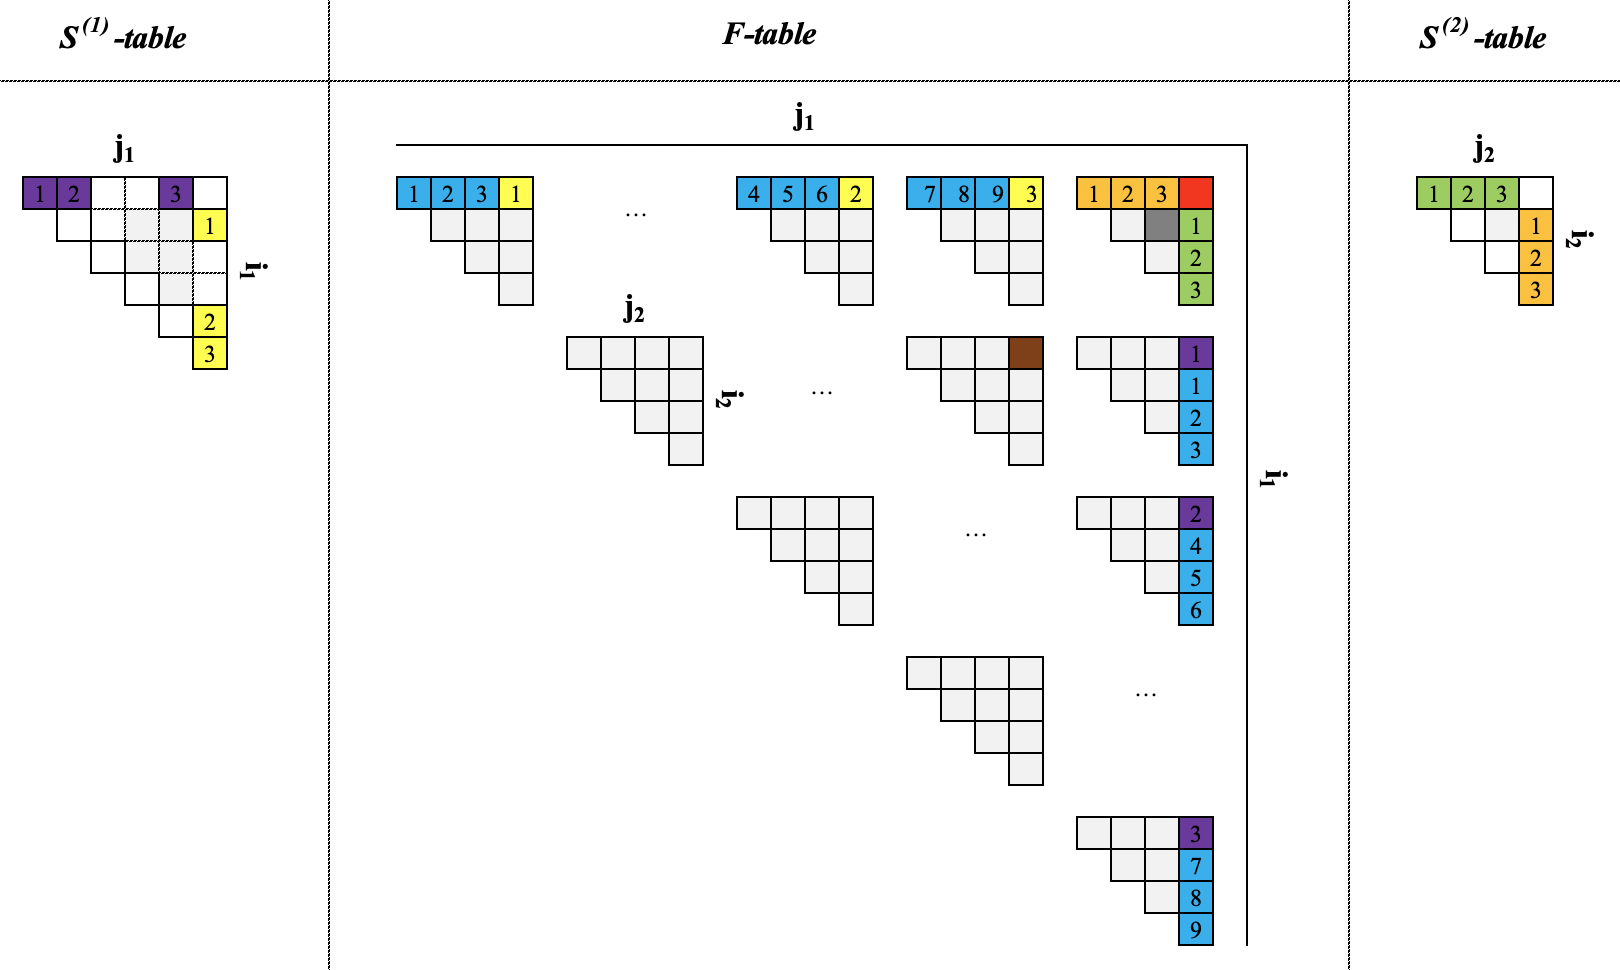
\includegraphics[scale=.30]{content/figures/bpm_dependency.png}}
\caption{BPMax dependency overview}
\label{fig:bpmax_dependency}
\end{figure}
Figure~\ref{fig:bpmax_dependency} shows the complete BPMax dependencies for an $F$-table element highlighted in red, which is dependent on all the blue, yellow, purple, orange, and green points of the $F$-table, $S^{(1)}$-table,  and $S^{(2)}$-table. Each color represents the computation of a particular reduction operation ($R^{0} - R^{4}$). %The blue, green, orange, purple, and yellow points contribute to the $R^{0}$, $R^{1}$, $R^{2}$, $R^{3}$, and $R^{4}$ respectively. 
All these reduction operations need to be completed to update the point highlighted in red. $R^{0}$ is the most compute-intensive ($\Theta({M^3N^3})$) reduction that uses the points outside the current triangle. E.g., To compute the $R^{0}$ for the red point,  the numbered blue points towards the left are added with the corresponding blue points towards the south, and then the max of all these values is computed. Now, $R^{3}$ and $R^{4}$ also use the elements from the external triangles as one of the operands and  $S^{(1)}$ as the other operand. E.g., the numbered yellow and purple points from the $F$-table are added with the corresponding yellow and purple points from the $S^{(1)}$-table, and then the max of yellow and purple results are computed to produce the $R^{3}$ and $R^{4}$, respectively. These two reductions have a $\Theta(M^3N^2)$ complexity. The remaining two reductions, $R^{1}$ and $R^{2}$, have a complexity of $\Theta(M^2N^3)$ and have intra-triangular dependencies. E.g., the numbered orange and green points from the $F$-table are added with the corresponding orange and green points from the $S^{(2)}$-table, and then the max of orange and green results are computed to produce the $R^{1}$ and $R^{2}$, respectively.




\subsection{Original Implementation} In the original BPMax implementation, all the diagonal elements are computed simultaneously, exposing the maximum level of parallelism. It accesses all the inner triangles  (highlighted in light red) towards the left of the diagonal points (red points Figure~\ref{fig:bpmax_original_schedule}). 
So, the total amount of the active data footprint required to compute all these points simultaneously can exceed the last-level cache for a larger input size, triggering a lot of data movement between different levels of caches and main memory. Memory reuse is almost impossible as we move to the next diagonal. Thus, the original program suffers from poor data locality.
\begin{figure}[htb]
\centerline{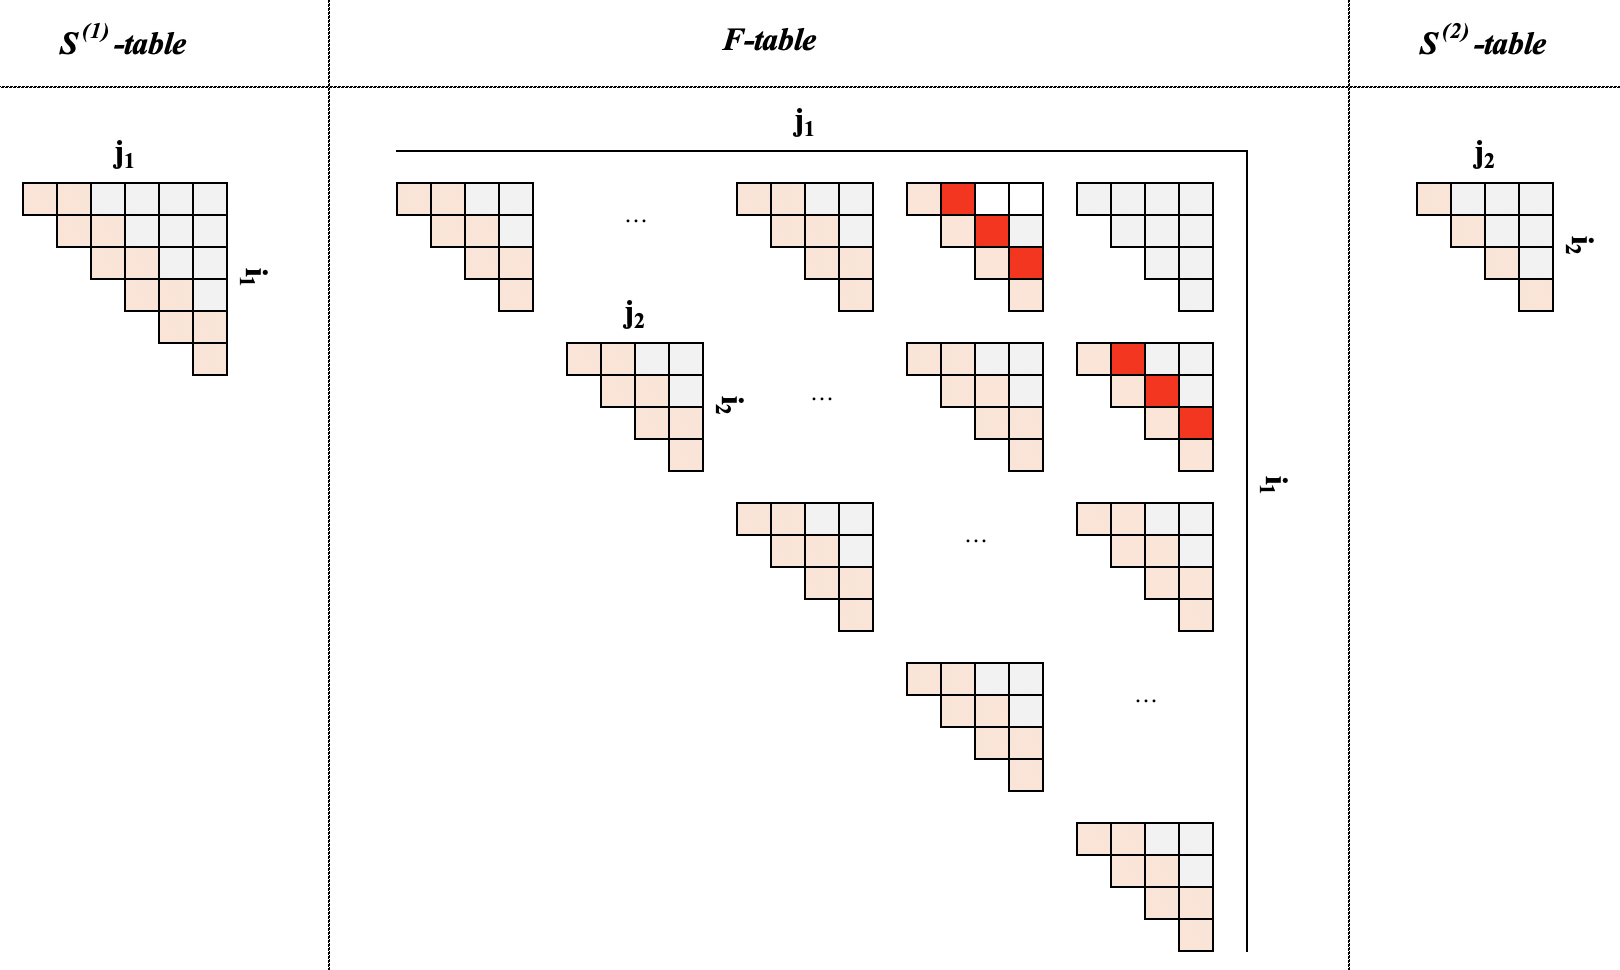
\includegraphics[scale=.30]{content/figures/bpmax_original_schedule.png}}
\caption{BPMax Original Schedule}
\label{fig:bpmax_original_schedule}
\end{figure}
Also, each of these reductions in the original implementation has loop carried dependencies, which prevents vectorization.

\subsection{Previous Optimization Approach} Our previous paper \cite{Mondal2021} introduced two levels of tiling to the BPMax - the first-level tilling to calculate each inner triangle at a time to improve the data locality. We also decomposed the double max-plus similar to \cite{Varadarajan2016} into a sequence of multiple matrix max-plus instances and applied loop tiling as the second-level tiling on each of the instances highlighted in Figure~\ref{fig:double_max_plus_accumulation_sequence_0}.
\begin{figure}[htbp]
\centering
\begin{subfigure}[b]{0.48\textwidth}
\centering
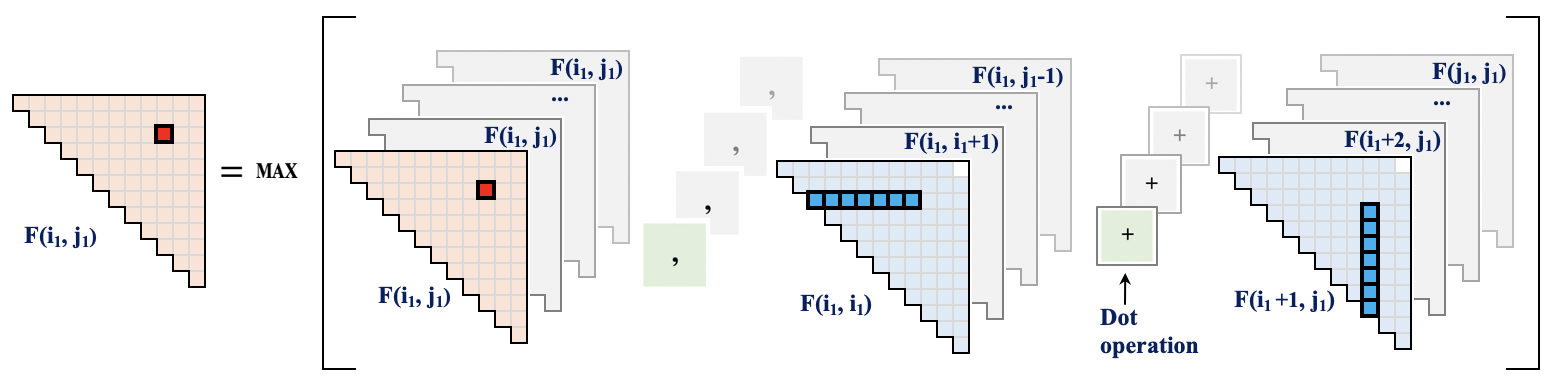
\includegraphics[scale=0.30, trim=4 4 4 4,clip]{content/figures/r0_1.png}
\caption{Decomposition of $R^{0}$}
\label{fig:double_max_plus_accumulation_sequence_0}
\end{subfigure}
\begin{subfigure}[b]{0.48\textwidth}
\vspace{1mm}
\centering
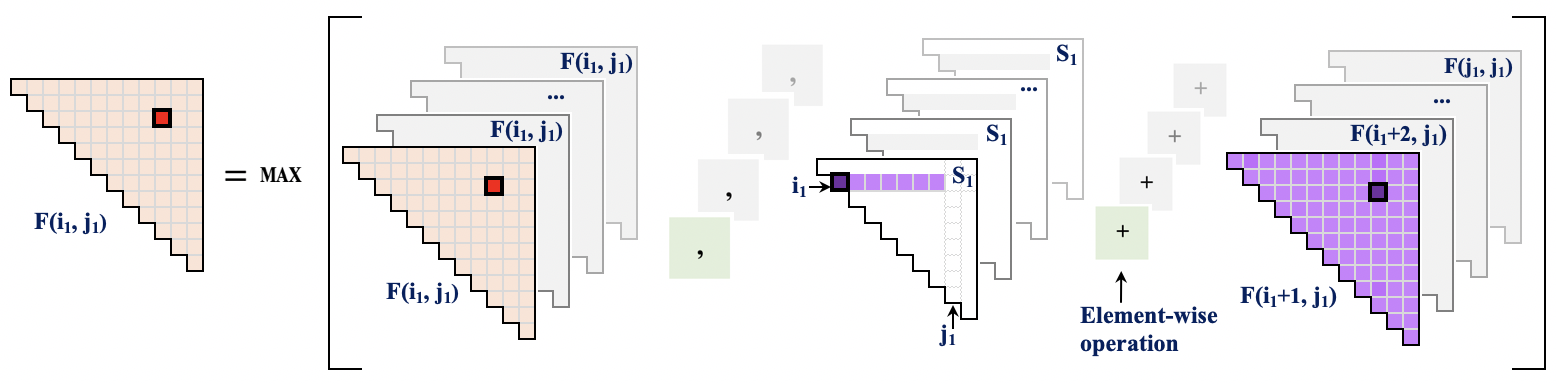
\includegraphics[scale=0.30, trim=4 4 4 4,clip]{content/figures/r3_1.png}
\caption{Decomposition of $R^{3}$}
\label{fig:R_3_optimization}
\end{subfigure}
\begin{subfigure}[b]{0.48\textwidth}
\vspace{1mm}
\centering
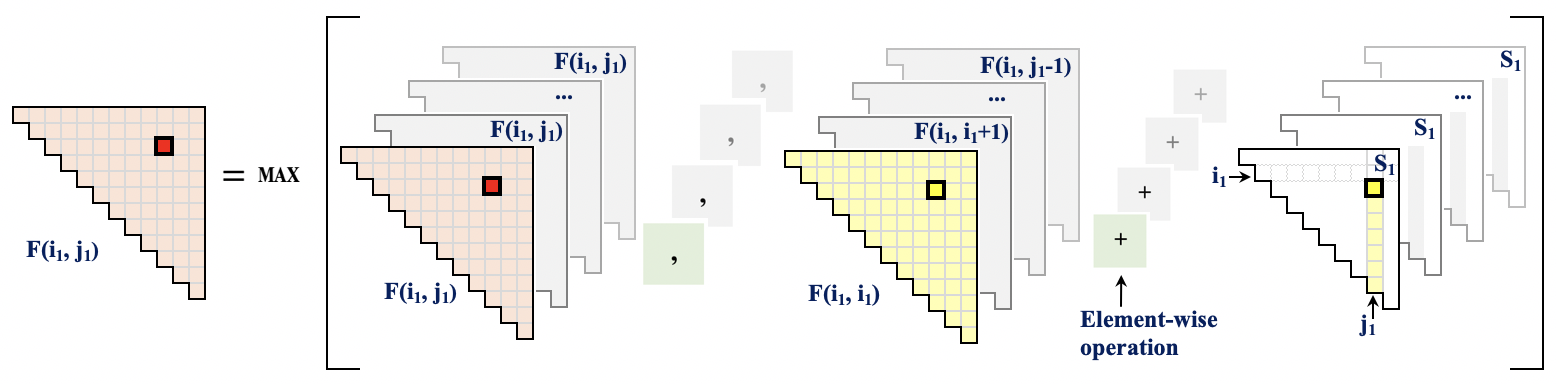
\includegraphics[scale=0.30, trim=4 4 4 4,clip]{content/figures/r4_1.png}
\caption{Decomposition of $R^{4}$}
\label{fig:R_4_optimization}
\end{subfigure}
\caption{$R^{0}$, $R^{3}$, and $R^{4}$ Accumulation}
\label{fig:bpm_outer_accumulation_sequence}
\end{figure}
We were able to tile each instance since there is no dependency between the input and output matrices. However, this approach had a few issues when we attempted to take advantage of auto-vectorization. It performed better only when the innermost dimension (vector dimension) was longer, which effectively prohibited the smaller tile dimension reducing better data locality. We noticed that $R^3$ requires the same inner triangles towards the south of $F(i_{1}, j_{1})$ and $S^{(1)}$, whereas $R^4$ requires the same inner triangles towards the west of $F(i_{1}, j_{1})$ and $S^{(1)}$ highlighted in Figure~\ref{fig:bpmax_dependency}. To take advantage of the re-use, we decomposed the $R^3$ similar to $R^0$ as a set of max-plus operations between $F$-table entries
(\{$F(k_{1}+1, j_{1}) \mid  i_{1} <=k_{1} < j_{1}$\}) 
and $S^{(1)}$ highlighted in Figure~\ref{fig:R_3_optimization}.
\begin{figure}[htbp]
\centering
\begin{subfigure}[htbp]{1\linewidth}
\centering
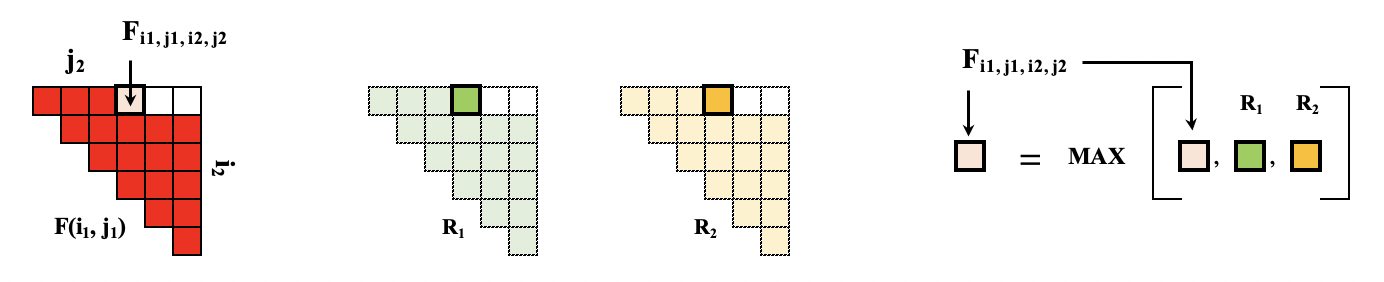
\includegraphics[scale=0.35, trim=4 4 4 4,clip]{content/figures/r0_r1_1.png}
\caption{Step 1: Let us assume that we are about to update the next element of $F(i_{1}, j_{1})$: $F_{i_{1}, j_{1}, i_{2}, j_{2}}$. Results of $R^{0}$, $R^{3}$, and $R^{4}$ corresponding to all the elements of $F(i_{1}, j_{1})$ are already accumulated in $F(i_{1}, j_{1})$. Let us also assume that  $R^{1}$ and $R^{2}$ are also computed for $F_{i_{1}, j_{1}, i_{2}, j_{2}}$ element. Thus, it gets updated with the maximum of the $F_{i_{1}, j_{1}, i_{2}, j_{2}}$,  $R^{1}$, and $R^{2}$.}
\label{fig:r3_r4_1}
\end{subfigure}
\begin{subfigure}[htbp]{1\linewidth}
\centering
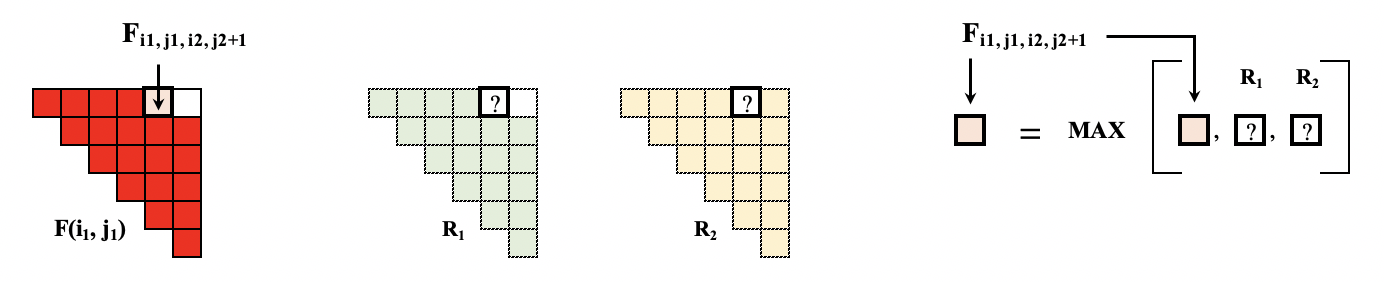
\includegraphics[scale=0.35, trim=4 4 4 4,clip]{content/figures/r0_r1_2.png}
\caption{Step 2: Next, we attempt to update $F_{i_{1}, j_{1}, i_{2}, j_{2} +1}$ highlighted in thick bordered light red box. 
%Results of $R^{0}$, $R^{3}$, and $R^{4}$ corresponding to this point is already available at $F_{i_{1}, j_{1}, i_{2}, j_{2} +1}$.  
$R^{1}$, and $R^{2}$ are not computed yet for $F_{i_{1}, j_{1}, i_{2}, j_{2} +1}$. Thus we need to compute these two reduction results before updating this point.}
\label{fig:r3_r4_2}
\end{subfigure}

\begin{subfigure}[htbp]{1\linewidth}
\centering
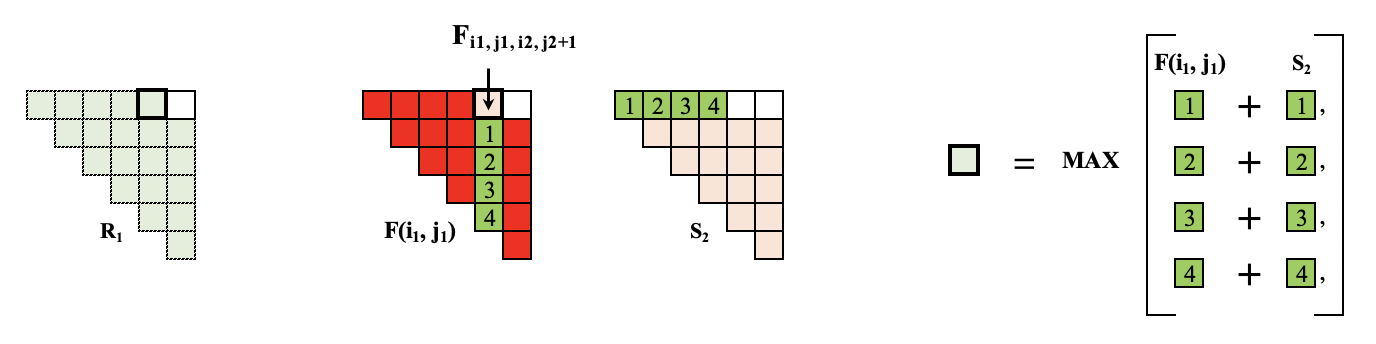
\includegraphics[scale=0.35, trim=4 4 4 4,clip]{content/figures/r0_r1_3.png}
\caption{Step 3: In this step, we compute  $R^{1}$ for $F_{i_1, j_1, i_2, j_2+1}$. It requires all the $F(i_1, j_1)$-table elements towards the south of $F_{i_1, j_1, i_2, j_2+1}$ and all the $S^{(2)}$-table elements towards the west of the corresponding $S^{(2)}$-table element.}
\label{fig:r3_r4_3}
\end{subfigure}


\begin{subfigure}[htbp]{1\linewidth}
\centering
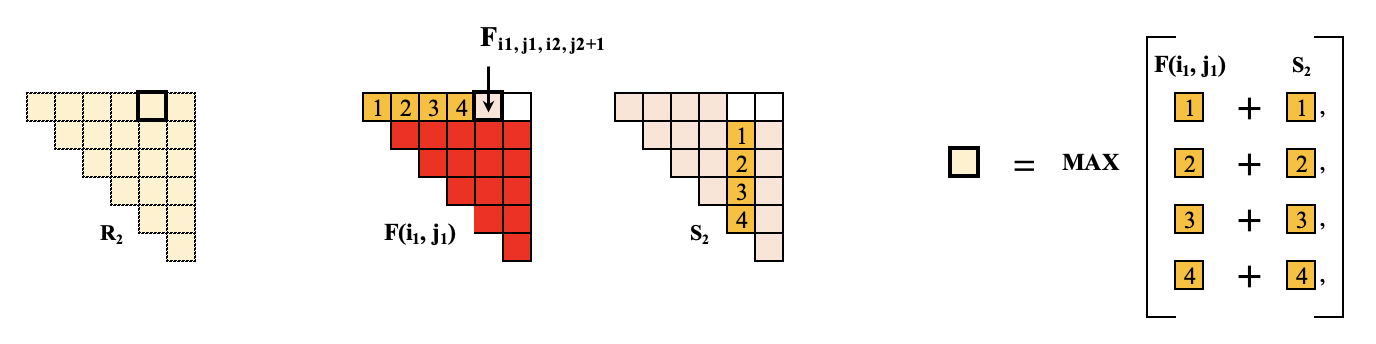
\includegraphics[scale=0.35, trim=4 4 4 4,clip]{content/figures/r0_r1_4.png}
\caption{Step 4: Now, we compute $R^{2}$ for  $F_{i_1, j_1, i_2, j_2+1}$. It requires all the $F(i_1, j_1)$-table elements towards the west of $F_{i_1, j_1, i_2, j_2+1}$ and all the $S^{(2)}$-table elements towards the south of the corresponding $S^{(2)}$-table element.}
\label{fig:r3_r4_4}
\end{subfigure}

\begin{subfigure}[htbp]{1\linewidth}
\centering
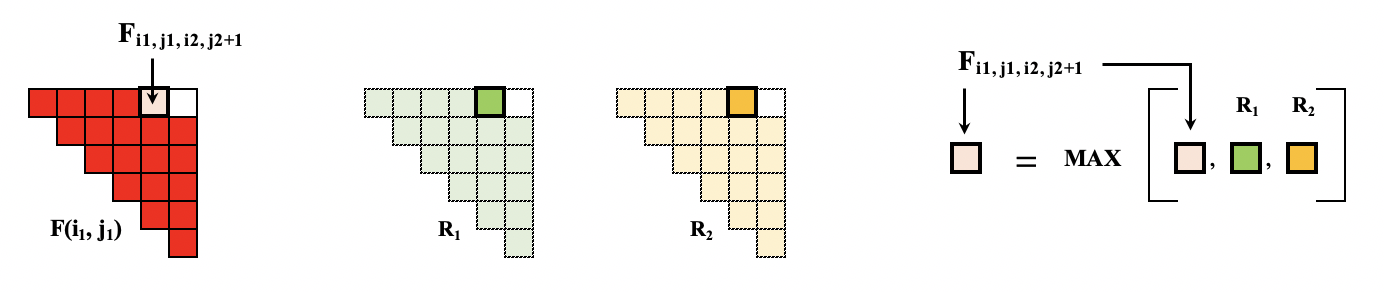
\includegraphics[scale=0.35, trim=4 4 4 4,clip]{content/figures/r0_r1_5.png}
\caption{Step 5: We have all the reduction results available at this point to update $F_{i_1, j_1, i_2, j_2+1}$. Next, we compute the $R^{1}$ and $R^{2}$ for updating the next $F$-table entry. This process continues until all the elements are updated.}
\label{fig:r3_r4_5}
\end{subfigure}
\caption{Illustration of $F$-table entry update with $R^{1}$ and $R^{2}$}
\label{fig:final_ftable_update}
\end{figure}
However, $R^3$ is an element-wise operation instead of the matrix product-like operations done in $R^{0}$. Similarly, $R^{4}$ can also be expressed as a set of element-wise max-plus operations between $S^{(1)}$ and $F$-table entries highlighted in Figure~\ref{fig:R_4_optimization}. After accumulating all the results from $R^{0}$, $R^{3}$, and $R^{4}$ into $F(i_{1}, j_{1})$, we updated it using $R^{1}$ and $R^{2}$. $R^{1}$ and $R^{2}$ have dependencies with the inner triangle that is being computed and $S^{(2)}$. Thus, these three updates must happen in a specific order demonstrated in Figure~\ref{fig:final_ftable_update}. Unlike $R^{0,3-4}$, we could not to tile these two reductions for each $F(i_{1}, j_{1})$. These are optimum string parenthesization (OSP)-like computations that require further transformation like middle serialization which were not trivial for our code generator. E.g., Simply pulling the reduction iteration($k_{2}$) from the innermost loop nest prohibits loop-tiling of the iteration space.


\subsection{New Optimization Strategy}
We introduce three levels of tiling in our new optimization strategy. The first-level tiling approach remains the same as our previous optimization approach, where we process each inner triangle as a tile. However, we take a different approach for the second-level tilling and introduce a third-level tiling highlighted in Figure~\ref{fig:bpmax_full_tiling}. The main objective behind the second and third-level tiles is to express most of the computation using small matrix-plus instances and then compute them in the most optimized way.

\begin{figure*}[htbp]
\centering
    \begin{subfigure}[htbp]{0.22\linewidth}
    \centering
    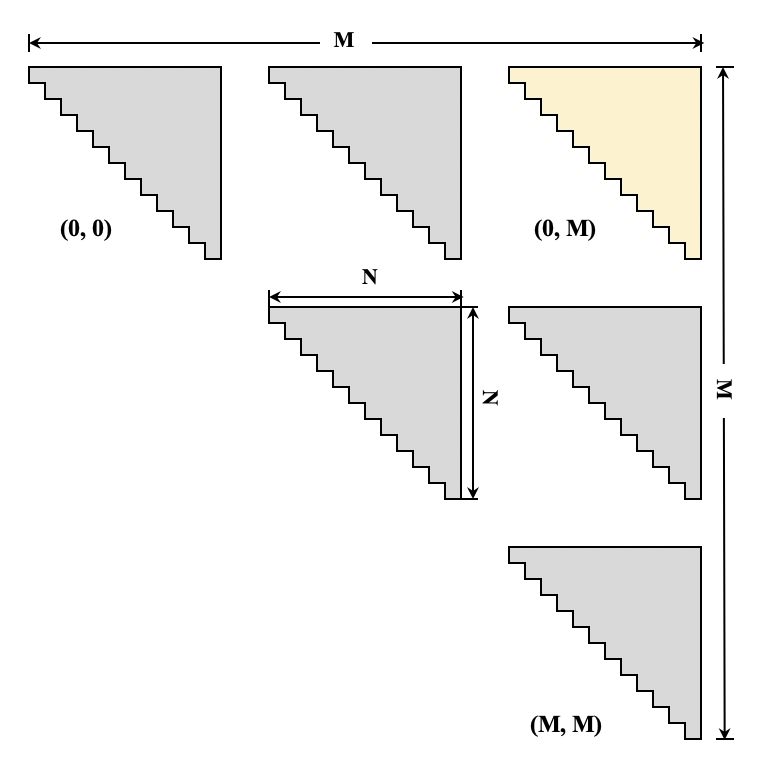
\includegraphics[scale=0.29, trim=2 2 2 2,clip]{content/figures/tile_0.png}
    \caption{FTable}
    \label{fig:tile_1}
    \end{subfigure}
    \begin{subfigure}[htbp]{0.22\linewidth}
    \centering
    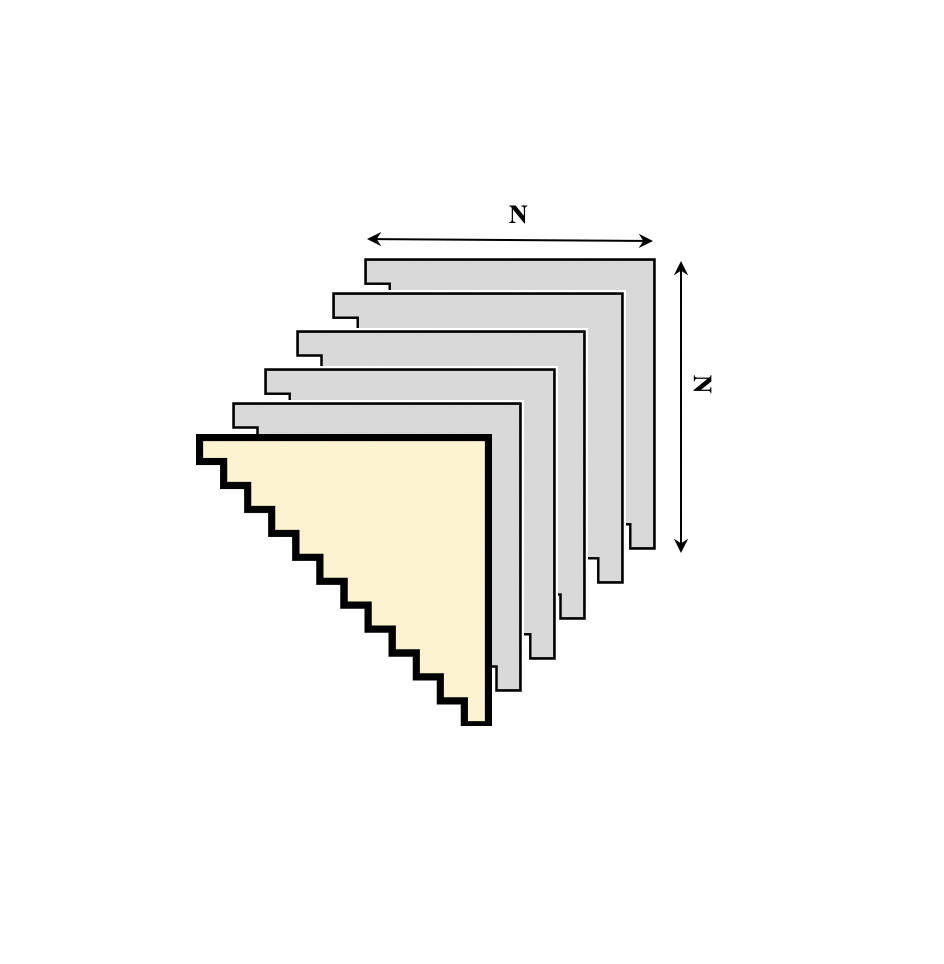
\includegraphics[scale=0.24, trim=2 2 2 2,clip]{content/figures/tile_1.png}
    \caption{Tile Level-I}
    \label{fig:tile_2}
    \end{subfigure}
    \begin{subfigure}[htbp]{0.22\linewidth}
    \centering
    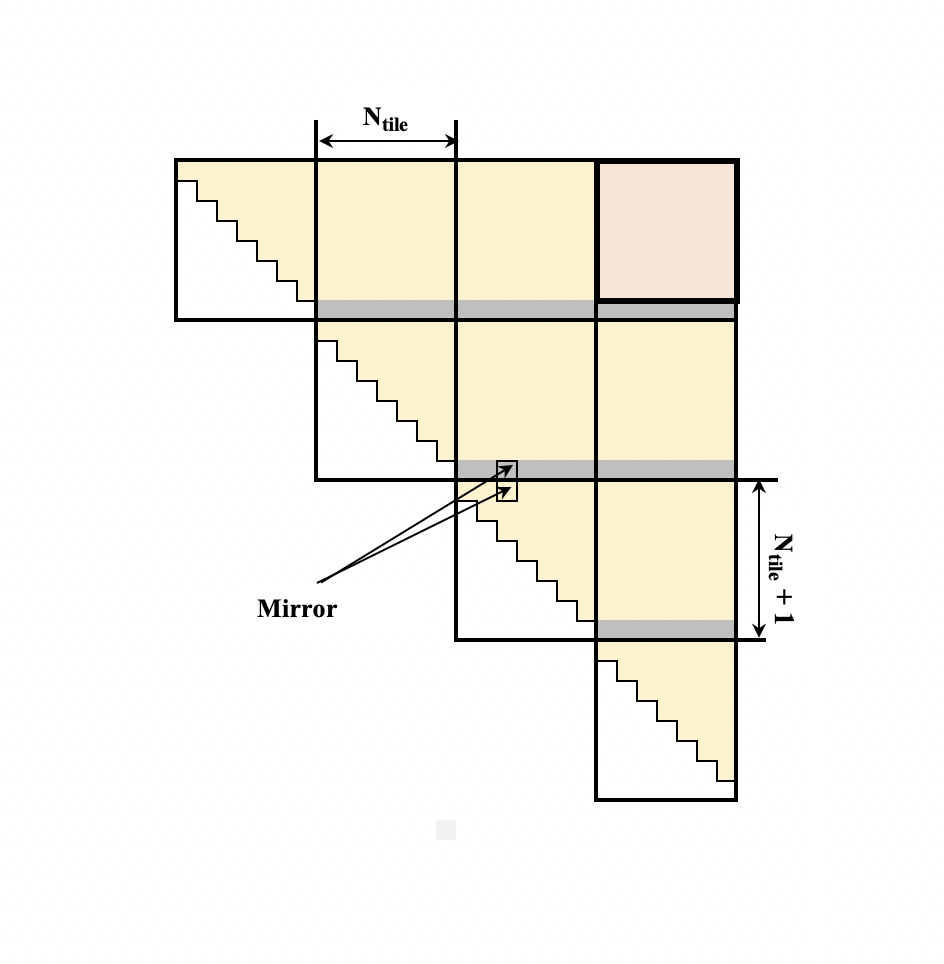
\includegraphics[scale=0.24, trim=2 2 2 2,clip]{content/figures/tile_2.png}
    \caption{Tile Level-II}
    \label{fig:tile_3}
    \end{subfigure}
    \begin{subfigure}[htbp]{0.22\linewidth}
    \centering
    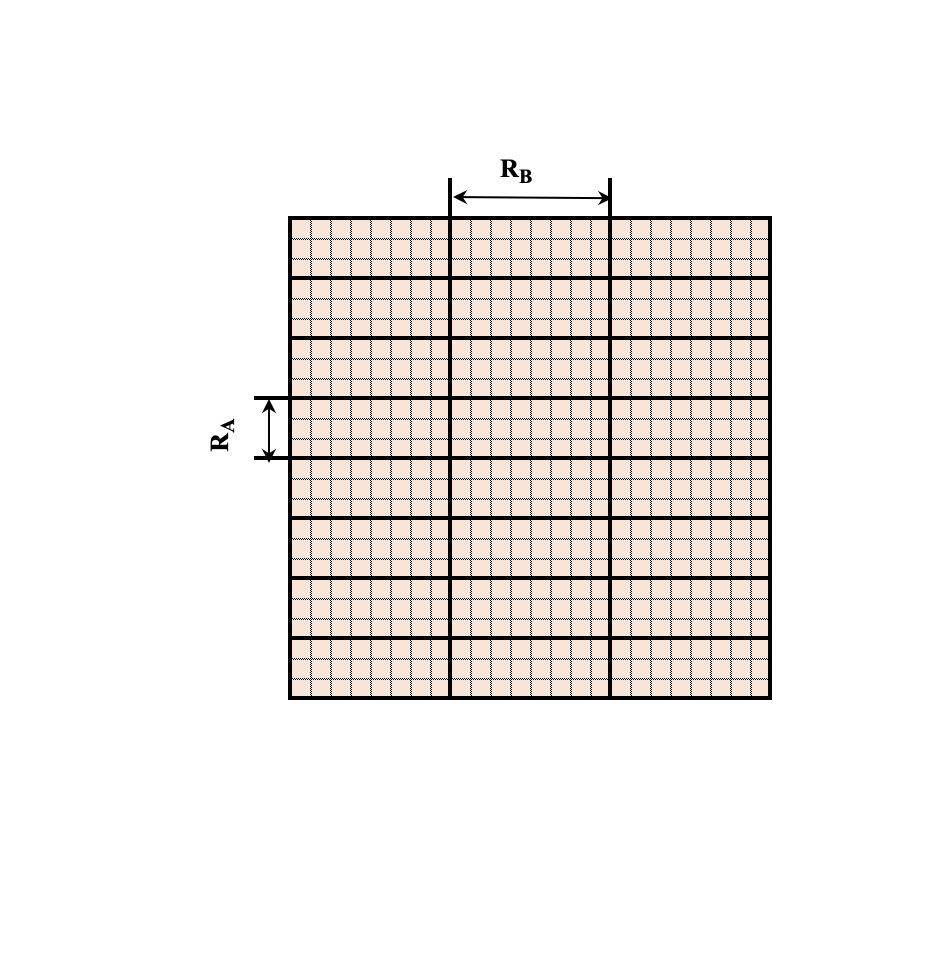
\includegraphics[scale=0.24, trim=2 2 2 2,clip]{content/figures/tile_3.png}
    \caption{Tile Level-III}
    \label{fig:tile_4}
    \end{subfigure}
\caption{Complete Tiling Overview: Computation granularity of the first-level tile ($N \times N$) is the inner triangle. The computation granularity of the second-level tile ($N_{tile+1} \times N_{tile}$) is the mono-parametric section of each inner triangle. Finally, the computation granularity of the third tiling level ($R_{A} \times R_{B}$) is the inner triangle subsection using registers.}
\label{fig:bpmax_full_tiling}
\end{figure*}

\subsubsection{Second-level Tiling}
The second-level tile divides the computation of each inner triangle based on mono-parametric tile size. It takes an input parameter $N_{tile}$ as a program input and partitions each inner triangle into multiple sections/tiles ($N_{sec}$) where, $N_{sec} =(N+N_{tile}-1) \div N_{tile}$,  $N$  = length of the second sequence (inner triangle). In other words, it introduces two new dimensions ($0 \le i_{2} \le j_{2} \le N_{sec}-1$ ) for each $F_{i_{1}, j_{1}, i_{22}, j_{22}}$ and transforms it to $F_{i_{1}, j_{1}, i_{2}, j_{2}, i_{3}, j_{3}} (i_{22}, j_{22} \mapsto i_{2}, j_{2}, i_{3}, j_{3})$. This transformation allows us to decompose the computations easily and schedule them efficiently using our code generation tool. Now, all the second-level diagonal tiles are triangular since they represent the edge of the inner triangle. We add additional elements to these and make them rectangular. These elements are initialized to the max identity value ($MIN\_FLOAT$). Each non-diagonal tiles are two dimensional ($i_{3}, j_{3}$) rectangular matrices. We add a row to each one of these tiles ($i_{2}, j_{2}$) to copy the first row of the tile ($i_{2+1}, j_{2}$). Thus the effective dimension of each one of second-level tile is $(N_{tile} +1) \times  N_{tile}$. It allows us to express all the BPMax reductions ($R^{0}, R^{1}, R^{2}, R^{3},$ and $R^{4}$) into many small matrix max-plus instances. Elements of each second-level tile are stored in row-major order, and the tiles themselves are stored in row-major order.

\begin{figure}
\centering
\begin{subfigure}[htbp]{0.48\textwidth}
\centering
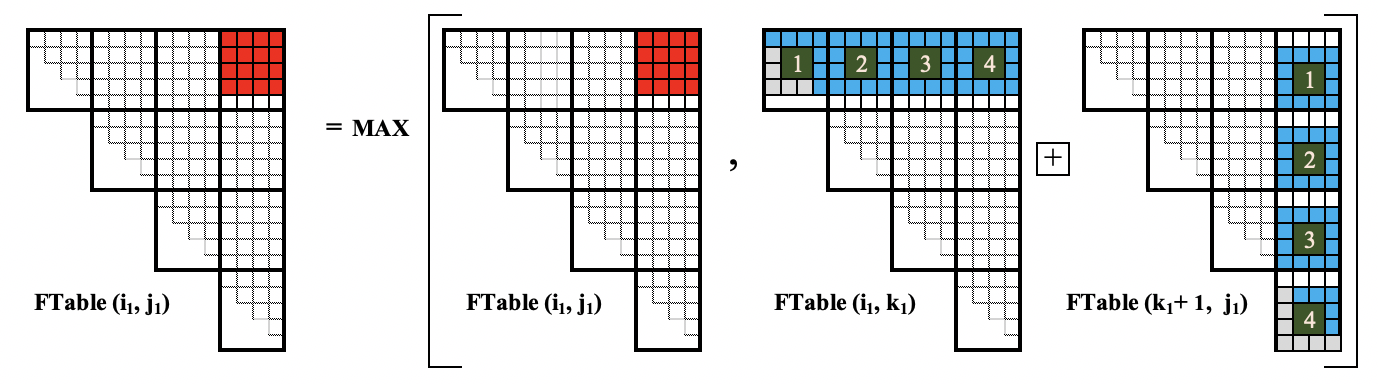
\includegraphics[scale=0.36, trim=4 4 4 4,clip]{content/figures/r0_mono_paramteric.png}
\caption{Second-level tiling of $R^{0}$}
\label{fig:mono_parametric_tile_r0}
\end{subfigure}
\hfill
\centering
\vspace{1mm}
\begin{subfigure}[htbp]{0.48\textwidth}
\centering
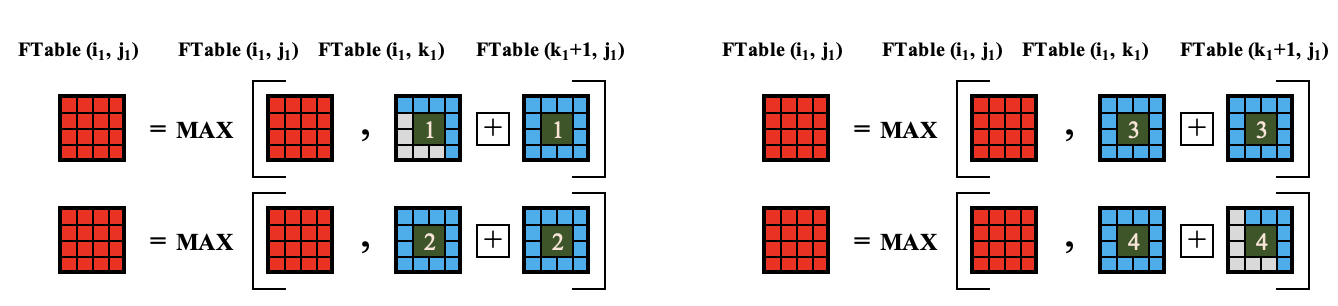
\includegraphics[scale=0.37, trim=4 4 4 4,clip]{content/figures/r0_max_plus.png}
\caption{Accumulation of $R^{0}$ using matrix max-plus}
\label{fig:matrix_max_plus_accum}
\end{subfigure}
\caption{Multi-level Decomposition of $R^{0}$}
\label{fig:rectangular_matrix_max_plus}
\end{figure}

\textbf{Mono-parametric Tiling of $R^{0}$:}
Mono-parametric tiling at the second-level transforms the original double max-plus into multiple matrix-plus operations.
Figure~\ref{fig:mono_parametric_tile_r0} shows a triangular matrix-max plus instance corresponding to a first-level tile, and Figure~\ref{fig:matrix_max_plus_accum} highlights the accumulation of a second-level tile (highlighted in red) using multiple small matrix max plus instances. The input and output tiles are distinct for each one of the second-level tile. Thus, the processing order could be either any row-major or column-major, or even reverse. It is possible to either accumulate the results for each output tile or process one tile at a time. If we compute each tile at a time, all the input tiles are used only once for computing the output, resulting in poor data locality. We avoid this by partially accumulating results for a tile by reusing one of the matrices, which is implemented using a second-level tile schedule.



\textbf{Mono-parametric Tiling of $R^{3}$ and $R^{4}$:}
Mono-parametric tiling at the second-level for $R^{3}$ and $R^{4}$ is important since they use the same inner triangles used in $R^{0}$. These are element-wise operations between $R^{0}$ input tiles and $S_{1}$. $R^{0}$, $R^{3}$, and $R^{4}$ reductions share some input tiles for a given output tile. Equation~\ref{eqn:r3_recurrence_mono} and~\ref{eqn:r4_recurrence_mono} highlights recurrence for a second-level tile corresponding to $R^{3}$ and $R^{4}$. Tiling these computations at the second-level allows us to schedule the second-level tiles such that they share the same input tiles between $R^{0}$, $R^{3}$, and $R^{4}$ and improve data locality.
\begin{equation}
\label{eqn:r3_recurrence_mono}
R^{(3)}_{i_{1},j_{1},i_{2},j_{2}, i_{3}, j_{3}} = 
    \max\limits_{k_{2}=i_{1}}^{j_{1}-1} S_{i_{1},k_{1}} + F_{k_{1}+1,j_{1}, i_{2}, j_{2}, i_{3}, j_{3}}\\
\end{equation}
\begin{equation}
\label{eqn:r4_recurrence_mono}
R^{(4)}_{i_{1},j_{1},i_{2},j_{2}, i_{3}, j_{3}} = 
    \max\limits_{k_{2}=i_{1}}^{j_{1}-1}  F_{i_{1},k_{1}, i_{2}, j_{2}, i_{3}, j_{3}} + S_{k_{1}+1,j_{1}}\\
\end{equation}


\textbf{Mono-parametric Tiling of $R^{1}$ and $R^{2}$:}
One of the significant advantages of the new second-level tiling is that it enables the transformation of the two inner reductions $R^{1}$, and $R^{2}$ corresponding to $F(i_{1}, j_{1})$ that significantly reduces complex atomic updates highlighted in Figure~\ref{fig:final_ftable_update}. After applying the second-level tile, we observe that each output tile has inter-tile and intra-tile dependencies. The inter-tile dependencies can be resolved by processing the tiles diagonally or bottom-up, and the intra-tile dependencies can be resolved using $R^{1}$, and $R^{2}$. Notice that majority of the $R^{1}$ and $R^{2}$ computations for each output tile can be transformed into several small matrix max-plus instances followed by a finalize phase that performs a small amount of $R^{1}$, and $R^{2}$. Like $R^{0}$ optimization, we can use a second-level tile schedule for these multiple matrices max-plus operations to reuse one of the input and partially accumulates results. 
\begin{figure}
\centering
\begin{subfigure}[b]{0.48\textwidth}
\centering
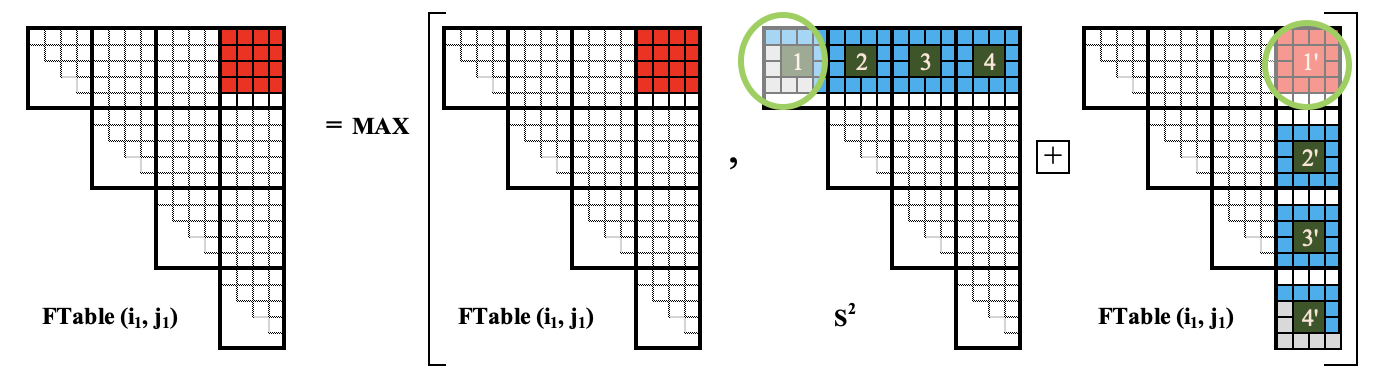
\includegraphics[scale=0.36, trim=4 4 4 4,clip]{content/figures/r1_top.png}
\label{fig:mono_r1_top}
\caption{Second-level Tiling of $R^{1}$}
\vspace{1mm}
\end{subfigure}
\centering
\begin{subfigure}[b]{0.48\textwidth}
\centering
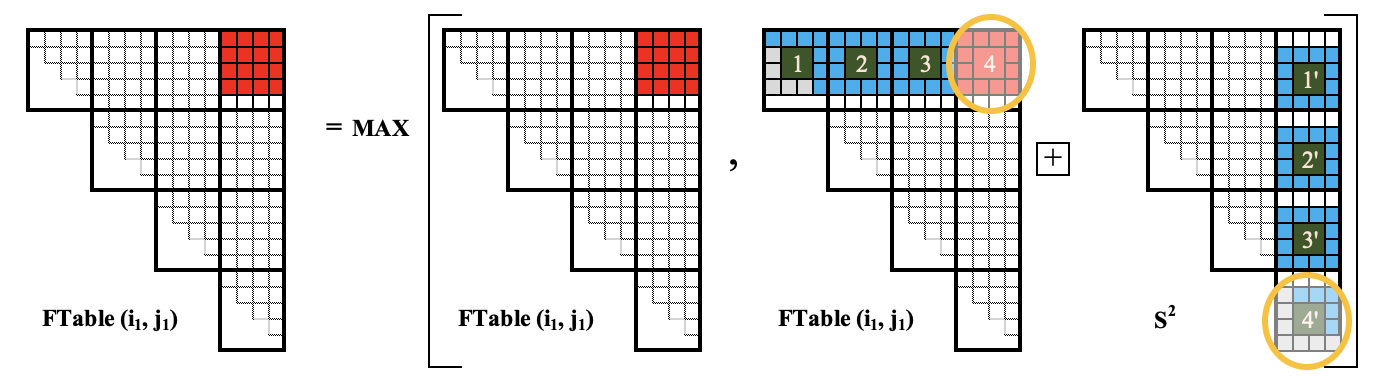
\includegraphics[scale=0.36, trim=4 4 4 4,clip]{content/figures/r2_top.png}
\caption{Second-level Tiling of $R^{2}$}
\label{fig:mono_r2_top}
\vspace{1mm}
\end{subfigure}
%\label{fig:r1_r2_optimization}
\begin{subfigure}[b]{0.22\textwidth}
\centering
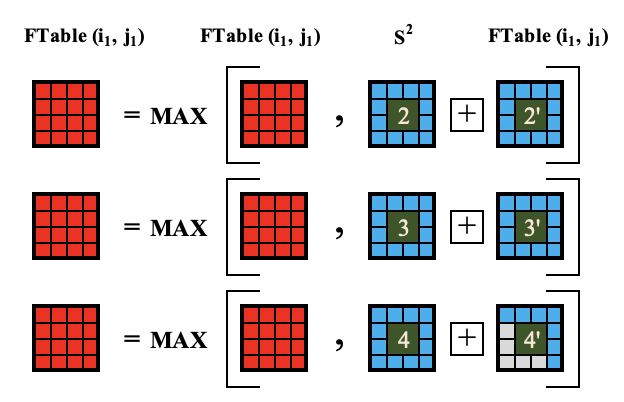
\includegraphics[width=\textwidth, scale=0.30, trim=4 4 4 4,clip]{content/figures/r1_max_plus.png}
\caption{$R^{1} \to$ Matrix max-plus}
\label{fig:R_1_matrix_max_plus}
\end{subfigure}
\vspace{0.5mm}
\begin{subfigure}[b]{0.22\textwidth}
\centering
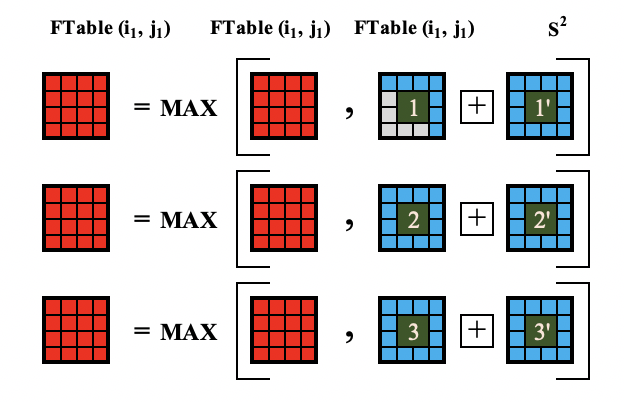
\includegraphics[width=\textwidth, scale=0.30, trim=4 4 4 4,clip]{content/figures/r2_max_plus.png}
\caption{$R^{2} \to$ Matrix max-plus}
\label{fig:R_2_matrix_max_plus}
\end{subfigure}
\begin{subfigure}[t]{0.22\textwidth}
\centering
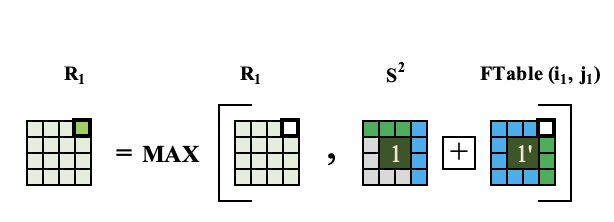
\includegraphics[width=\textwidth, scale=0.30, trim=4 4 4 4,clip]{content/figures/r1_finalize.png}
\caption{Residual $R^{1}$ }
\label{fig:mono_R_1}
\end{subfigure}
\begin{subfigure}[t]{0.22\textwidth}
\centering
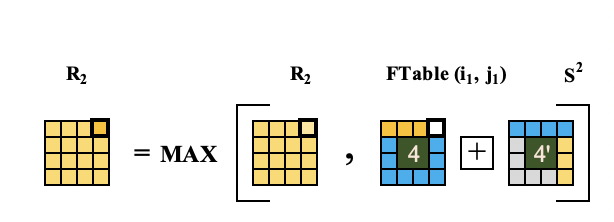
\includegraphics[width=\textwidth, scale=0.30, trim=4 4 4 4,clip]{content/figures/r2_finalize.png}
\caption{Residual $R^{2}$}
\label{fig:mono_R_2}
\end{subfigure}
\vspace{0.5mm}
\begin{subfigure}[t]{0.22\textwidth}
\centering
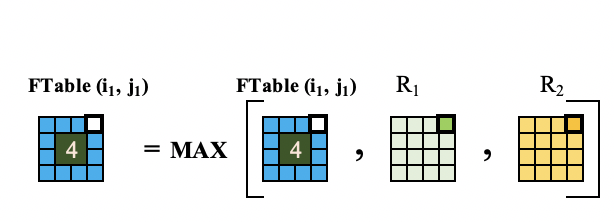
\includegraphics[width=\textwidth, scale=0.30, trim=4 4 4 4,clip]{content/figures/ftable_final.png}
\caption{Final Update}
\label{fig:mono_final}
\end{subfigure}
\caption{Multi-level Decomposition of $R^{1}$ and $R^{2}$}
\label{fig:R_1_2_matrix_max_plus}
\end{figure}
Besides finalize phase, the diagonal tiles also require the $R^{1}$ and $R^{2}$ recurrences and use the same steps highlighted in Figure~\ref{fig:final_ftable_update}.
Figure~\ref{fig:R_1_2_matrix_max_plus} show how a tile of $F(i_{1}, j_{1})$ is computed by transforming the computations into many small matrix max-plus problem instances and residual computations before making the final update.


\subsubsection{Third-level Tiling}

Second-level tiling allows us to improve data locality significantly. Now, we can rely on the vectorization process to improve CPU resource utilization and reduce L1 bandwidth by a factor of SIMD width. However, further optimization is required to reduce the L1 bandwidth and achieve maximum CPU utilization. So, we apply the register-blocking/tiling (\textbf{RT}), where we compute a patch (third-level tile) of the second-level tile that fits in the vector register. Elements from the input matrices are loaded into the memory and used multiple times to update the patch, effectively reducing the memory accesses for the input and output.

\begin{figure}[htbp]
\centerline{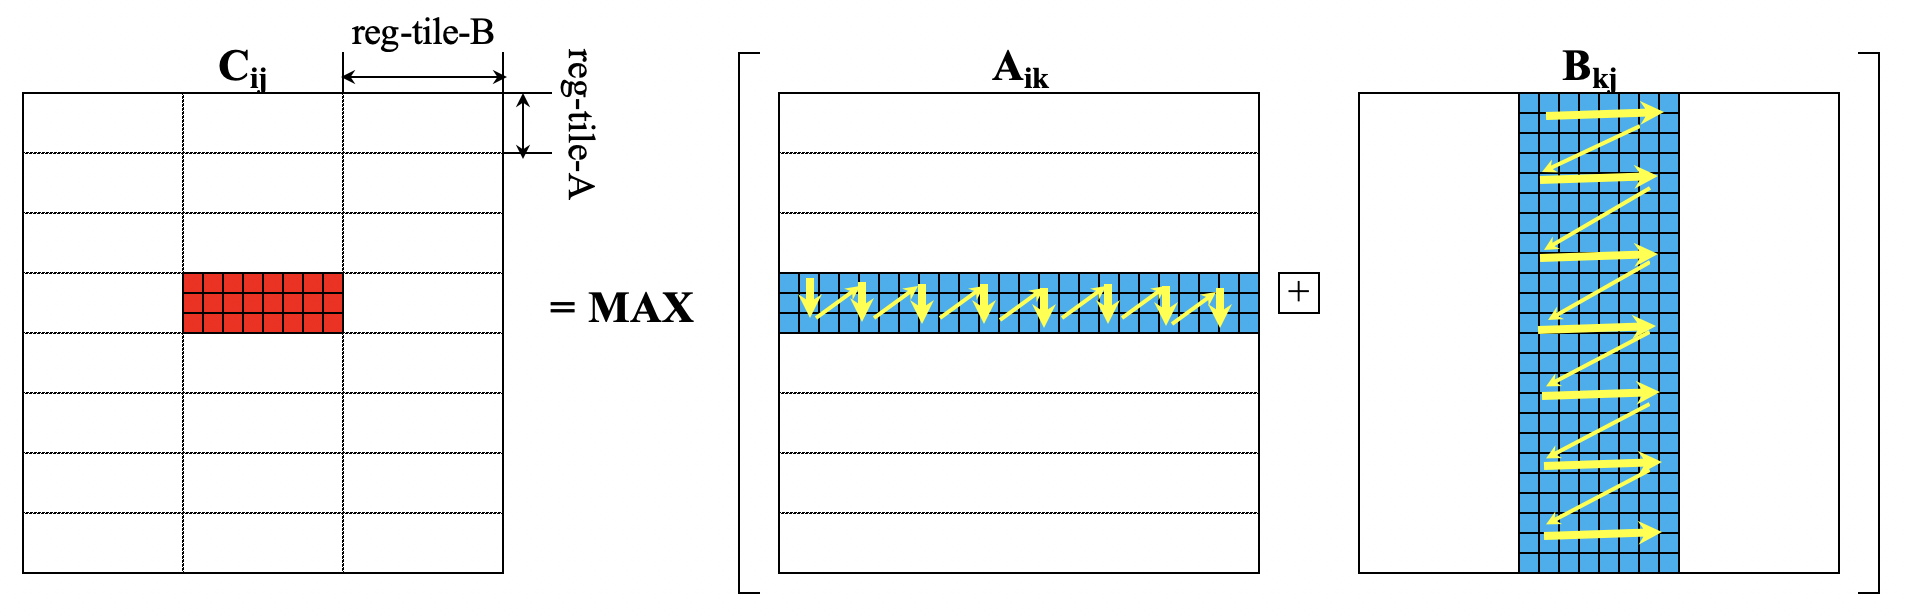
\includegraphics[scale=0.25, trim=5 5 5 5,clip]{content/figures/register_tile.png}}
\caption{Register Tiling (\textbf{RT})}
\label{fig:regiser_tile}
\end{figure}

Sequential memory access is a well-known property of any modern CPU-specific register-tiled kernel. Its performance depends on how the scalar and vector inputs are read from the memory and their alignments. So, we transform the first input matrix (let us call this A) and the second input matrix (let us call this B) such that the memory access pattern from the register-tile kernel is sequential. Figure~\ref{fig:regiser_tile} shows the memory access pattern of our register tile. Previously, similar techniques were also implemented for a register tile that performed FMA operations by Huang et al. \cite{FLAWN80}. We observe that an inner-$F$-table triangle or $S_{2}$ can be used several times as a $A$ or $B$ operand. Thus, it is possible to transform each triangle with two different memory layouts once and avoid transforming the same tile multiple times. 

\subsubsection{Buffer Transformation Strategy}
We have explored three buffer transformation techniques for accessing data sequentially within the register-tiled code. They are based on when we transform \textbf{register-tile-operand-A} and \textbf{register-tile-operand-format-B}. The first one \textbf{ [MPT+RT]:v1} transforms each inner $F$-table and $S_{2}$ to \textbf{register-tile-operand-A} and \textbf{register-tile-operand-format-B} exactly once but  introduces four new $F$-table variables - $F(A)$,  $F(B)$, $S_{2}(A)$, $S_{2}(B)$ in the system. The inner reductions $R_{1}$ and $R_{2}$ also use $S_{2}$ as the other operand for the max-plus operation. \textbf{ [MPT+RT]:v2} uses on-the-fly transformation for both of the operands, and \textbf{[MPT+RT]:v3} uses pre-transformed $S_{2}$ but transforms the inner $F$-table on the fly. 





\textbf{Parallelization Strategy:} We process the first-level tiles diagonally and assign all the cores to a first-level tile to accumulate the results from each instance of outer reductions - $R^{0}$, $R^{3}$, and $R^{4}$. Each core is responsible for processing all the second-level tiles of a particular row. It helps the cores share the input and out inner triangles in the L3 cache. After all the first-level tiles in a diagonal is accumulated from outer reductions, we assign each core to update the first-level tile with the inner reductions - $R^{1}$, $R^{2}$. 



















\section{Implementation}\label{sec:implementation}
\IEEEPARstart{I}{n} In this section, we present the code generation process using \alphaz\ and key insights into some of our implementation techniques. We discuss the formulation of different schedules, implementation of different optimization strategies with the \alphaz, and optimization of matrix max-plus handwritten kernel. 
\subsection{\alphaz\ }\label{sec:alphaz}
\alfa~\cite{Mauras1989} is a strongly typed functional language based on
%\todo{awk} 
systems of affine recurrence equations defined over polyhedral domains. It was developed by Mauras~\cite{Mauras1989}  in 1989.  Subsequently, it was extended to include subsystems and reductions~\cite{leverge-thesis, leverge-parle92, fdupont-asap96, florent-thesis, DupontQuRi93}. \alphaz\ is a tool that allows program transformations and user-directed compilation of \alfa\ programs.  It provides a general framework for analysis, transformation, and code generation in the polyhedral equational model.  \alphaz\ is similar to an earlier tool - \textsc{\texttt{MMAlpha}} ~\cite{guillou-mma} , which targets field-programmable gate array-based hardware design. On the other hand, \alphaz\ targets code generation for multiprocessor shared-memory programs and focuses on programs with reduction operations. 


Most of the polyhedral code optimization tools use hard-coded transformation strategies and generate code automatically. But the performance of such code often falls short of a hand-written optimized version. To avoid fixed transformation strategies, tools like Chill~\cite{Chen08chill:a}, Hailde~\cite{RaganKelley2013}, and \alphaz\ ~\cite{sanjay-lcpc2012} implement various code transformation APIs and present them to the users. It allows users to choose different transformations for a specific problem, enabling a large exploration space for the optimization process.

\begin{figure}[htbp]
\centerline{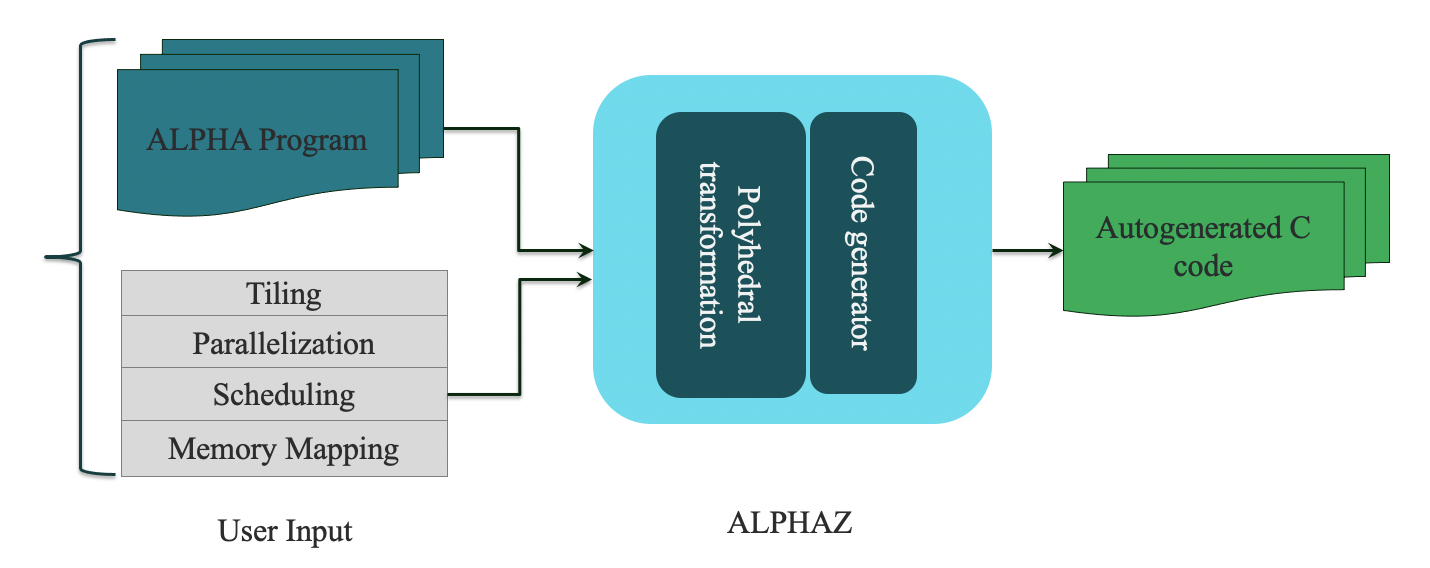
\includegraphics[scale=0.35,trim=5 5 5 5,clip]{content/figures/code_generation_methodology.png}}
\caption{Code generation methodology}
\label{fig:code_gen_methodlogy}
\end{figure}
\alphaz\ code optimization process has two parts – input specification and compilation script.  Input specification allows a user to express the computation using mathematical equations. The compilation script takes inputs (e.g., scheduling, parallelization, memory-mapping, and tiling transformations) from the user to generate optimized C code corresponding to the input specification. Figure~\ref{fig:code_gen_methodlogy} highlights the code optimization methodology using \alphaz\ .  


All the transformations in \alphaz\ are semantics preserving. However, it is the user's responsibility to ensure the transformations are valid. We use three important classes of transformations - target mappings, memory mappings, and tiling-related transformations. Target mappings-related transformations determine the execution order of the program. It allows the user to specify schedule and processor allocation for each variable in the system. It also allows the user to specify one or more dimensions of the schedule to be executed in parallel by different threads.  Memory mappings-related transformations allow multiple variables with different dimensions to share the same memory map based on the affine function. It also allows multiple variables with the same dimension to share memory space. Tiling transformations chop the iteration space to improve data locality and adjust parallelization granularity. Target and Memory mappings-related transformations require the user to specify the affine functions to indicate the schedule or memory map. The affine functions are expressed as $(ListOfIndices \mapsto ListOfIndexExpressions)$.
\begin{itemize}
    \item A schedule $(i, j \mapsto j, i)$ tells \alphaz\ that the iteration domain is $2$-dimensional represented by $i$, $j$ as the $ListOfIndices$, and the points in this iteration domain should be visited in the order given by the $ListOfIndexExpression$   $j$ and $i$.
    \item A memory map $(i, j \mapsto j, i)$ tells \alphaz\ that the mapping is associated with a $2$-D variable whose $(i, j)$-th element is stored at a location specified by $ListOfIndexExpressions$ - $(j, i)$.  It also allows the user to save memory if there is an opportunity for many-to-one mapping. E.g., $(i, j, k \mapsto i, j)$.
\end{itemize}

Efficient scheduled code generation depends on the choice of target and memory mappings-related transformations. 
Algorithm~\ref{algo:matrix_mul_alphabets} highlights the \alfa\ program for matrix multiplication. Algorithm~\ref{algo:matrix_mul_script} presents a compiling script for matrix multiplication that produces the C code highlighted in Listing~\ref{listing:alpha_code_gen}.


\begin{algorithm}
\caption{Matrix Multiplication in Alphabets}
\begin{algorithmic} [1]
\STATE \textbf{affine} MM $\lbrace N,K,M \mid (M, N, K)  > 0  \rbrace$
\STATE \textbf{input}
\STATE  \hspace{10pt} float A $\lbrace i, j \mid 0 \leq i < M \hspace{2pt} \&\& \hspace{2pt} 0 \leq j < K   \rbrace$ ;
\STATE  \hspace{10pt} float B $\lbrace i, j \mid 0 \leq i < K \hspace{2pt} \&\& \hspace{2pt} 0 \leq j < N   \rbrace$ ;
\STATE \textbf{output}
\STATE  \hspace{10pt} float C $\lbrace i, j \mid 0 \leq i < M \hspace{2pt} \&\& \hspace{2pt} 0 \leq j < N   \rbrace$;
\STATE \textbf{local}
\STATE \hspace{10pt} \slash \slash \text{local variables}
\STATE \textbf{output}
\STATE \hspace{10pt} C[$i,j$] = reduce(+, \hspace{2pt} [$k$], \hspace{2pt} A[$i,k$] * B[$k,j$]);
\end{algorithmic}
\label{algo:matrix_mul_alphabets}
\end{algorithm}
\begin{algorithm}
 \caption{Matrix Multiplication Command Script}
 \begin{algorithmic} [1]
 \STATE \text{\slash \slash \hspace{2pt}$Step-1: Parse \hspace{2pt} Alphabet \hspace{2pt} $}
 \STATE \text{prog=ReadAlphabets("MM.ab");}
 \STATE \text{system = “MM”;}
 \STATE \text{outDir="./src";}

 \STATE \text{}
 \STATE \text{\slash \slash \hspace{2pt}$Step-2: Perform \hspace{2pt} polyhedral \hspace{2pt}  transformation$}
 \STATE \text{Normalize(prog);}
 \STATE \text{setSpaceTimeMap(prog,  system,  “C”,  }
 \STATE \text{.  "($i,j,k \mapsto i, k, j$)", “($i,j \mapsto i, -1, j$)”); }
 \STATE \text{setParallel(prog,  system,  “”,  "0" );}
 \STATE \text{}
 \STATE \text{\slash \slash \hspace{2pt}$Step-3: Generate  \hspace{2pt} code$}
 \STATE \text{generateWriteC(prog,  system,  outDir);}
\STATE \text{generateScheduleC(prog,  system,  outDir);}
\end{algorithmic}
\label{algo:matrix_mul_script}
\end{algorithm}

\newpage
\begin{lstlisting}[label={listing:alpha_code_gen}, language=Caml, caption=Generated code - Matrix multiplication]
#define S1(i,j,i2) C(i,i2) = 0.0
#define S0(i0,i1,i2) C(i0,i2) = 
(C(i0,i2))+((A(i0,i1))*(B(i1,i2)))
{
    int c1,c2,c3;
    #pragma omp parallel for private(c2,c3)
    for(c1=0;c1 <= M-1;c1+=1){
	   for(c3=0;c3 <= N-1;c3+=1){
	       S1((c1),(-1),(c3));
	   }
       for(c2=0;c2 <= K-1;c2+=1){
            for(c3=0;c3 <= N-1;c3+=1){
                S0((c1),(c2),(c3));
            }
        }
    }
}

\end{lstlisting}


\textbf{Subsystems:} One of the primary challenges of using a polyhedral code generator is to produce readable, modular code. \alphaz\ subsystem construct is handy for addressing this. It helps organize a complex \alfa\ program into different parts capable of taking one or more \alfa\ variables as input to produce an output. \alphaz\ treats the subsystem itself like a variable to allow the user to specify a schedule for controlling the invocation and a memory map for optimizing variable passing between subsystem caller and callee. The subsystem invocations can be precisely controlled for any point in the iteration space.





\subsection{Previous BPMax Schedules}
\textbf{Original BPMax Schedule:}
Let us recall that the original BPMax computed a four-dimensional table $F$-table based on five reductions ($R^{0}$, $R^{1}$, $R^{2}$, $R^{3}$, $R^{4}$) and two two-dimensional tables - $S^{(1)}$ and $S^{(2)}$. \alphaz\ treats each of these entities as a unique variable and requires the user to specify a schedule and a memory map. We have observed previously that $S^{(1)}$ and $S^{(2)}$ require only the input sequences. Thus, they can be scheduled before any other reductions. The schedules of the remaining variables are formulated based on the wavefront parallelization of the 6-D schedule space. We highlight the original program schedule in Table~\ref{tab:bpm_original_schedule}.
\begin{table}[htbp]
\caption{\uppercase{BPMax original Parallelization}}
\begin{center}
\begin{tabular}{|c|c|}
\hline
\textbf{\textit{Reduction}}& \textbf{\textit{Schedules}} \\
\hline
$S^{(1)}$ & $(i_{1},j_{1}, k_{1} \mapsto  0, j_{1}-i_{1}, i_{1}, k_{1}, 0, 0, 0)$   \\
\cline{1-2} 
$S^{(2)}$ & $(i_{2},j_{2}, k_{2} \mapsto  0, j_{2}-i_{2}, i_{2}, k_{2}, 1, 1, 1)$   \\
\cline{1-2} 
$R^{0}$ & $(i_{1},j_{1},i_{2},j_{2},k_{1},k_{2} \mapsto 1, j_{1}-i_{1}, j_{2}-i_{2}, i_{1}, i_{2}, k_{1}, k_{2})^{\mathrm{a}}$    \\
 \cline{1-2} 
$R^{1}, R^{2}$ & $(i_{1},j_{1},i_{2},j_{2},k_{2} \mapsto 1, j_{1}-i_{1}, j_{2}-i_{2}, i_{1}, i_{2}, k_{2}, 0)^{\mathrm{a}}$   \\
\cline{1-2} 
$R^{3}, R^{4}$ & $(i_{1},j_{1},i_{2},j_{2},k_{1} \mapsto 1, j_{1}-i_{1}, j_{2}-i_{2}, i_{1}, i_{2}, k_{1}, 0)^{\mathrm{a}}$ \\
 \cline{1-2} 
\hline
\multicolumn{2}{l}{$^{\mathrm{a}}$Parallel Dimension 3 (1-based)}
\end{tabular}
\label{tab:bpm_original_schedule}
\end{center}
\end{table}

We also recall the most optimized schedule from our prior work ~\cite{Mondal2021} shown in Table~\ref{tab:hybrid_schedule_with_tiling}.


\begin{table}[htbp]
\caption{\uppercase{BPMax hybrid schedule with tiling}}
\begin{center}
\begin{tabular}{|c|c|c|}
\hline
\textbf{} & \textbf{\textit{Variable}}& \textbf{\textit{Schedule}} \\
\hline
 &  Output & $(i_{1},j_{1} \mapsto M, i_{1}, j_{1}, 0)$ \\
 \cline{2-3} 
${\mathrm{a}}$ & $R_{0}$ & $(i_{1},j_{1},k_{1},k_{2} \mapsto k_{1}, i_{1}, k_{2}, j_{1})$,    \\
\cline{2-3} 
& $R_{3}, R_{4}$ & $(i_{1},j_{1},k_{1} \mapsto k_{1}, i_{1}, i_{1}, j_{1})$    \\
% \cline{2-3} 
\hline
%\cline{2-3} 
& a & $(i_{1},j_{1} \mapsto 1, j_{1}-i_{1}, i_{1}, j_{1}-4, 0, 0, 0)$   \\
\cline{2-3} 
${\mathrm{b}}$ & $F$ & $(i_{1},j_{1},i_{2},j_{2} \mapsto 1, j_{1}-i_{1}, M, i_{1}, -i_{2}, j_{2}, 0)$   \\
\cline{2-3} 
& $R_{1}, R_{2}$ & $(i_{1},j_{1},i_{2},j_{2},k_{2} \mapsto 1, j_{1}-i_{1}, M, i_{1}, -i_{2}, k_{2}, j_{2})$  \\
% & & $(i_{1},j_{1},i_{2},j_{2} \mapsto 1, j_{1}-i_{1}, M, i_{1}, -i_{2}, i_{2}-1, j_{2})$ \\
\hline
%\multicolumn{3}{l}{}\\
\multicolumn{3}{l}{${\mathrm{a}}$ - Subsystem schedule(parallel dimension 1)}\\
\multicolumn{3}{l}{${\mathrm{b}}$ - Root system schedule(parallel dimension 3)}\\
\end{tabular}
\label{tab:hybrid_schedule_with_tiling}
\end{center}
\end{table}


\subsection{New BPMax Schedules}
We used the BPMax equation as specified in the original paper ~\cite{EbrahimpourBoroojeny2021} in our previous optimization work ~\cite{Mondal2021}. In our current optimization work, we manually transform the original BPMax equations to apply the second and third-level tiling based on a mono-parametric tile parameter and develop a modified \alfa program. It allows precise scheduling, memory mapping, and transformations of the second-level tiles. We express various computations using subsystems and apply optimization on each of them independently to produce modular code.

Similar to the prior optimization work, we compute the $S^{(1)}$ and $S^{(2)}$ table first. However, we apply mono-parametric tiling on $S^{(2)}$ so that we can use a second-level tile as one of the matrix max-plus operands for computing $R^{1}$ and  $R^{2}$. Let us now discuss the $F$-table schedules at the different tiling levels.

\textbf{First-level Tile Schedule:}
Each first-level tile (an inner triangle) goes through different computation phases (point-wise operations and reductions) associated with a unique subsystem. The point-wise operations initialize (subsystem - $Initialization$) the $F$-table and update (subsystem - $Point\-wise^{sw}$) using the inner triangle to its south-west. Subsystem - $Reductions^{outer}$ accumulates the result from the outer reductions - $R^{0}$, $R^{3}$, $R^{4}$ and subsystem - $Reductions^{inner}$ makes the final update to each tile using the inner reductions - $R^{1}$, $R^{2}$. We process diagonal tiles one at a time for invoking point-wise operations ($Initialization$ and $Point\-wise^{sw}$) and outer reductions $Reductions^{outer}$. $Reductions^{outer}$ accumulates the results from a set of $F(i_{1}, k_{1})$ and $F(k_{1}+1, j_{1})$ triangles where $i_{1} \le k_{1} < j_{1}$.  $2^{nd}$ and $3^{rd}$ dimensions of these subsystem's schedules control the diagonal processing order. \begin{table}[htbp]
\caption{\uppercase{First Level Tile Schedule}}
\begin{center}
\begin{tabular}{|c|c|}
\hline
\textbf{\textit{Subsystem}}& \textbf{\textit{Schedule}}$^{\mathrm{a}}$ \\
\hline
$S^{(1)}, S^{(2)}$ & $(i_{1} \mapsto 0, 0, i_{1}, 0, 0, 0, 0)$   \\
\cline{1-2} 
%\hspace{5mm}
$Initialization$ & $(i_{1},j_{1},i_{2},j_{2} \mapsto 2, j_{1}-i_{1}, i_{1}, -1, i_{2}, j_{2},0)$   \\
\cline{1-2} 
%\hspace{5mm}
$Point\-wise^{sw}$ & $(i_{1},j_{1},i_{2},j_{2} \mapsto 2, j_{1}-i_{1}, i_{1}, -1, i_{2}, j_{2},1)$   \\
\cline{1-2}
$Reductions^{outer}$ & $(i_{1},j_{1},k_{1} \mapsto 2, j_{1}-i_{1}, i_{1}, k_{1}, 0, 0, 0)$    \\
\cline{1-2}
$Reductions^{inner}$ & $(i_{1},j_{1},k_{1} \mapsto 2, j_{1}-i_{1}, M, 0, i_{1}, 0, 0)$    \\
 \cline{1-2} 
\hline
%\multicolumn{2}{l}{}\\
\multicolumn{2}{l}{$^{\mathrm{a}}$Parallel dimension 5}
\end{tabular}
\label{tab:tile_l1}
\end{center}
\end{table}
Notice that initialization of the entire $F$-table is costly due to its footprint. So, we schedule $Initialization$ and $Point\-wise^{sw}$ together ($5^{th}$ and $6^{th}$ dimension of the schedule) before scheduling the $Reductions^{outer}$ (ordering is controlled by the $4^{th}$ dimension of the schedule). After completing all the outer reductions, we schedule $Reductions^{inner}$ ($3^{rd}$ dimension greater than $M-1$) for multiple tiles simultaneously. Table~\ref{tab:tile_l1} outlines the schedule for each one of these subsystems along with $S^{(1)}$ and $S^{(2)}$. The parallel dimension 5 indicates that multiple threads are assigned to do point-wise operations on a particular tile, whereas each tile is finalized ($Reductions^{inner}$) by one thread.


\textbf{Second-level Tile Schedule:} Second-level tiles are processed by $Reductions^{outer}$ and $Reductions^{inner}$ subsystems. $Reductions^{outer}$ accumulates partial results for all the second-level tiles $\{ i_{2}, j_{2} \mid 0 \le i_{2} \le j_{2} \le N_{sec}-1 \}$ for a given first-level tile $F(i_{1}, j_{1})$. It is responsible for scheduling $R^{3}$ (subsystem - $R^{3}_{t}$), $R^{4}$ (subsystem - $R^{4}_{t}$), multiple matrix max-plus input transformations (subsystem - $MT(F)^{A}$ and $MT(F)^{B}$), and multiple matrix max-plus computations (subsystem - $MMP$). For matrix max-plus operation, each second-level tile $F(i_{1}, j_{1}, i_{2}, j_{2})$ is updated using a set of input tiles $F(i_{1}, k_{1}, i_{2}, k_{2})$ and $F(k_{1}+1, j_{1}, k_{2}, j_{2})$ where $i_{2} \le k_{2} \le j_{2}$. As noted earlier, instead of evaluating one output tile at a time, we use a schedule that accumulates results in the output tile. Since $R^{0}$, $R^{3}$, $R^{4}$ share the input tiles, we first schedule the $R^{3}_{t}$ and $R^{4}_{t}$ and reuse the input tiles in $MMP$. We schedule $MT(F)^{A}$ to transform an input tile and use it multiple times as the first operand in a $MMP$ invocation. Before each $MMP$ invocation, we schedule $MT(F)^{B}$ to transform the second operand of the matrix max-plus operation. Table~\ref{tab:bpm_l2_outer_reduction_schedule} highlights the schedule for the different subsystems invoked from $Reductions^{outer}$.
\begin{table}[htbp]
\caption{\uppercase{Second Level Tile, Outer Reductions}}
\begin{center}
\begin{tabular}{|c|c|c|}
\hline
&\textbf{\textit{Subsystem}}& \textbf{\textit{Schedule}}$^{\mathrm{b}}$ \\
\hline
&$R^{3}_{t}$, $R^{4}_{t}$ & $(i_{2},j_{2} \mapsto 0, i_{2},j_{2}, 0, 0, 0)$   \\
\cline{1-3} 
 &$MT(F)^{A}$  & $(i_{2},j_{2} \mapsto 0, i_{2},j_{2}, 0, 0, 1)$   \\
\cline{2-3} 
${\mathrm{a}}$ &$MT(F)^{B}$  & $(i_{2},j_{2},k \mapsto 0, i_{2}, k_{2}, 1, j_{2}, 0)$   \\
\cline{2-3} 
&$MMP$ ($R^{0}$) & $(i_{2},j_{2},k_{2} \mapsto 0, i_{2}, k_{2}, 1, j_{2}, 1)$   \\
\hline
\multicolumn{3}{l}{${\mathrm{a}}$ - Optimized $R_{0}$}\\
\multicolumn{3}{l}{${\mathrm{b}}$ - Parallel dimension 5}
\end{tabular}
\label{tab:bpm_l2_outer_reduction_schedule}
\end{center}
\end{table}

 
\begin{table}[htbp]
\caption{\uppercase{Second Level Tile, Inner Reductions}}
\begin{center}
\begin{tabular}{|c|c|c|}
\hline
\textbf{} & \textbf{\textit{Subsystem}}& \textbf{\textit{Schedule}} \\
\hline
 & $Diagonal Tile$ & $(i_{2},j_{2} \mapsto -i_{2}, j_{2}, 0, j_{2}, 0)$   \\
\cline{2-3} 
\hline
%\cline{2-3} 
 & $MT(S^{2})^{A}$ & $(i_{2},j_{2} \mapsto -i_{2}, j_{2}, 0, j_{2}, 1)$   \\
\cline{2-3} 
${\mathrm{a}}$ & $MT(F)^{B}$ & $(i_{2},j_{2},k_{2} \mapsto -i_{2}, k_{2}, 3, j_{2}, 0)$    \\
 \cline{2-3} 
 &  $MMP$ ($R_{1}$) & $(i_{2},j_{2},k_{2} \mapsto -i_{2}, k_{2}, 3, j_{2}, 1)$ \\
\hline
 & $MT(F)^{A}$ & $(i_{2},j_{2} \mapsto -i_{2}, j_{2}, 4, j_{2}, 0)$    \\
\cline{2-3} 
${\mathrm{b}}$ & $MT(S^{2})^{B}$ & $(i_{2},j_{2},k_{2} \mapsto -i_{2}, k_{2}, 5, j_{2}, 0)$    \\
 \cline{2-3} 
 & $MMP$ ($R_{2}$) & $(i_{2},j_{2},k_{2} \mapsto -i_{2}, k_{2}, 5, j_{2}, 1)$ \\
\hline
& $Finalize$ & $(i_{2},j_{2} \mapsto -i_{2}, j_{2}, 0, j_{2}, 0)$ \\
\hline
\multicolumn{3}{l}{${\mathrm{a}}$ - Optimized $R_{1}$}\\
\multicolumn{3}{l}{${\mathrm{b}}$ - Optimized $R_{2}$}\\
\end{tabular}
\label{tab:bpm_l2_inner_reduction_schedule}
\end{center}
\end{table}


$Reductions^{inner}$ subsystem takes a first-level tile $F(i_{1}, j_{1})$ and $S_{2}$ as input and makes the final update to the $F(i_{1}, j_{1})$. It is responsible for scheduling a diagonal tile (subsystem - $DiagonalTile$), optimized $R_{1}$ (subsystem - $MT(S^{2})^{A}$, $MT(F)^{B}$, $MMP$), optimized $R_{1}$ ($MT(F)^{A}$, $MT(S^{2})^{B}$, $MMP$) and residual patch up computation ($Finalize$). Table~\ref{tab:bpm_l2_outer_reduction_schedule} highlights a bottom-up and left-to-right schedule for these subsystems. So, we first schedule the $DiagonalTile$ tile corresponding to each tile row. For each non-diagonal tile, we schedule all the subsystems that optimize the $R^{1}$, followed by $R^{2}$. Scheduling these subsystems is similar to optimizing $R^{0}$. Finally, we schedule $Finalize$ for each non-diagonal tile to resolve the intra-tile dependencies.

\begin{table*}[htbp]
\caption{\uppercase{Register allocation Strategy}}
\label{tab:ymm_registers}
\begin{center}
\begin{tabular}{|c|c|c|c|c|c|c|c|c|}
\hline
Number & Number & Number of& Number of & Number of YMMs & Total &Number of & Number of   \\
of A & of B & YMMs for A & YMMs for  B&  for accumulations&YMMs Usage &Memory access&  Max-plus  Operations(v)\\
\hline
2 & 24 & 2 & 3 & 6 & 11  & 5 & 6 \\
\hline
2  & 32 & 2 & 4 & 8 & 14 & 6 & 8  \\
\hline
3 & 24 & 3 & 3 & 9 & 15  & 6 & 9 \\
\hline
3 & 16 & 3 & 2 & 6 & 11 & 5 & 6  \\
\hline
4 & 16 & 4 & 2 & 8 & 14  & 6 & 8  \\
\hline
\end{tabular}
\end{center}
\end{table*}

\textbf{Third-level Tile Schedule:}
 We implement the third-level tile using an optimized hand-written register-tiled kernel that performs matrix max-plus. We process the third-level register tile in a column-major order ($i_{3}, j_{3} \mapsto {j_3}, i_{3}$).  The design of the register-tiled kernel is target-dependent. We use Intel intrinsic APIs to compute multiple max-plus operations using Intel Advanced Vector Extensions (AVX-256) registers.

Due to many architectural similarities, we use a common register-tiling implementation for our target architectures - Broadwell and Coffee Lake architecture. One of the main differences between these two architectures is the number of available floating-point addition units (FPA) per core. Even though both architectures have two floating-point multiply-add (FMA) units, Broadwell has only one floating-point add unit, whereas Coffee Lake has two floating-point add units. Since the max operation is also executed using the FPA unit and the number of instructions per cycle for vaddps and vmaxps are twice smaller for Broadwell than Coffee Lake,  Broadwell architecture is significantly bottle-necked for the max-plus computation. The objective of the register tiling is to load the data into the registers and perform as many operations as we can without accessing memory. AVX-256 has sixteen 256-bit registers YMM0-YMM15, which perform a single instruction on multiple data elements. Each YMM register can hold eight single-precision floating points and be used to store operands or results to perform eight single-precision operations. The execution latency of vaddps and vmaxps operation on Coffee Lake is four cycles (3 for the Broadwell). Thus, we need to have 8 (6 for the Broadwell) independent chains of computations to fully utilize both FPA execution ports for Coffee Lake.

We are interested in a data access pattern of $C = (a + B) \max C $, where $a$ is a scalar and $B$, $C$ are vectors. So, we load eight consecutive elements (vector) of $B$ and $C$ into the YMM registers (B, C) but load a single element (scalar) of $a$ and broadcast it to a YMM register(A). The goal is to find the combination of $A$ and $B$ that maximizes CPU-resource utilization. Table~\ref{tab:ymm_registers} shows the different register tiles ($ A\times B$) that maximize the resource utilization but minimize the AVX register allocation. We notice that $3 \times 24$ maximizes the resource utilization with the best memory access to compute ratio. 

\textbf{Memory Access:} We implement several techniques to optimize memory access. Each core is responsible for executing a complete matrix max-plus operation that requires data transformation. We use a dedicated buffer for these transformations and select them using omp\_get\_thread\_num(). We ensure the processor-to-memory affinity by setting OMP\_PLACES to 'cores' and set OMP\_PROC\_BIND to true to bind the OMP threads to the physical core to improve data locality during the on-the-fly memory transformation. We use Intel intrinsic for allocating these transformation buffers so that they are aligned to SIMD width ($8 \times 4$ bytes).







\section{Result}\label{sec:result}
\IEEEPARstart{W}{e} present our results with two intel target architectures - Xeon E-2278G and Xeon E5-1650v4. Both architectures run AlmaLinux 8.5, where we have performed our experiments. Table 4.1 highlights the CPU properties. We use Intel compiler ICC 19.1.3.304 with -O3  -qopenmp -xCORE-AVX2 -ipo options as a compiler flag.

\begin{table}[htbp]
\caption{\uppercase{CPU Parameters Overview}}
\label{tab:cpu parameters}
\begin{center}
\begin{tabular}{|c||c|c|}
\hline
 Parameters & Xeon E5-1650v4  & Xeon E-2278G \\
\hline
\hline
Micro-Architecture & Broadwell  & Coffee Lake \\
\hline
Number of cores & 6 & 8  \\
Number of threads & 12 & 16  \\
\hline
Base Frequency (GHz) & 3.6  & 3.4  \\
Turbo Frequency (GHz) & 4.0 & 5.0   \\
\hline
L1 Cache (KB) - Per Core  & 32 & 32  \\
L2 Cache (KB) - Per Core &  256  & 256 \\
L3 Cache (MB) - Shared & 15 & 16 \\
DRAM (GB) & 16 & 32 \\
\hline
\end{tabular}
\end{center}
\end{table}


Our optimized BPMax uses single-precision floating point. We measure the performance by calculating the number of single-precision floating-point operations executed per second (FLOPS). Now, GFLOPS indicates $10^9$ floating-point operations per second. Although GFLOPS is typically used to highlight double-precision performance, we will use this terminology to denote the single-precision performance in the rest of our discussion. We first present the theoretical machine peak, then the roofline machine peak measured by the Intel Advisor before presenting the performance of the Double max-plus and BPMax.

\subsection{Max-plus Machine Peak Analysis}
We calculate the theoretical CPU machine peak using the following equation:
\begin{equation}\label{eqn:machine_peak_eqn}
\begin{split}
\text{Single-precision Machine Peak (GFLOPS)} &= \\
\text{Number of vector operations} \times \text {Instructions per cycle} \times \\
\text{Number of Cores} \times \text{Core Frequency (GHz)} \\
\end{split}
\end{equation}


Table~\ref{tab1:Theoretical_machine_peak} highlights the theoretical machine peak of our target architectures. The theoretical max-plus machine peak of Coffee Lake and Broadwell are $435.2$ and $172$ GFLOPS, respectively when the cores run at the base frequency.

\begin{table*}[htbp]
\caption{\uppercase{Max-plus Theoretical Machine Peak}}
\label{tab1:Theoretical_machine_peak}
\begin{center}
\begin{tabular}{|c|c|c|c|c|c|}
\hline
 & Number &  Frequency &  Instructions & Machine Peak Single Core (GFLOPS)& Machine Peak Total\\
 Processor & of Cores& (GHz)  & per cycle & (GFLOPS) & (GFLOPS)\\
  & &  [Base, Turbo] & [add, max]  & [Base, Turbo] & [Base, Turbo]\\
\hline
Xeon E5-1650v4 & 6 & [3.6, 4.0] & [1, 1] & [28.8, 32] & [172.8, 192] \\
\hline
Xeon E-2278G & 8 & [3.4, 5.0] & [2, 2] & [54.4, 80] & [435.2, 640] \\
\hline
%\multicolumn{5}{l}{}
\end{tabular}
\end{center}
\end{table*}


\textbf{Arithmetic Intensity of BPMax:} BPMax computation can be summarized as $ Y = max(a + X, Y)$.  It uses three single-precision memory accesses to perform two arithmetic operations (max and plus). So, its arithmetic intensity (AI) is $\frac{2}{(3\times4)}$or $\frac{1}{6}$ FLOPS/byte.

\textbf{Coffee Lake Roofline}: Figure~\ref{fig:roof_line_coffee_lake} shows the max-plus roofline collected on the Coffee Lake machine using the Intel Advisor tool. We observe that the attainable max-plus machine peak of Coffee Lake in our environment is around 585 GFLOPS, which is significantly lower than the theoretical max-plus machine peak of 640 GLOPS with the processor running at maximum frequency.

\begin{figure}[htbp]
\centerline{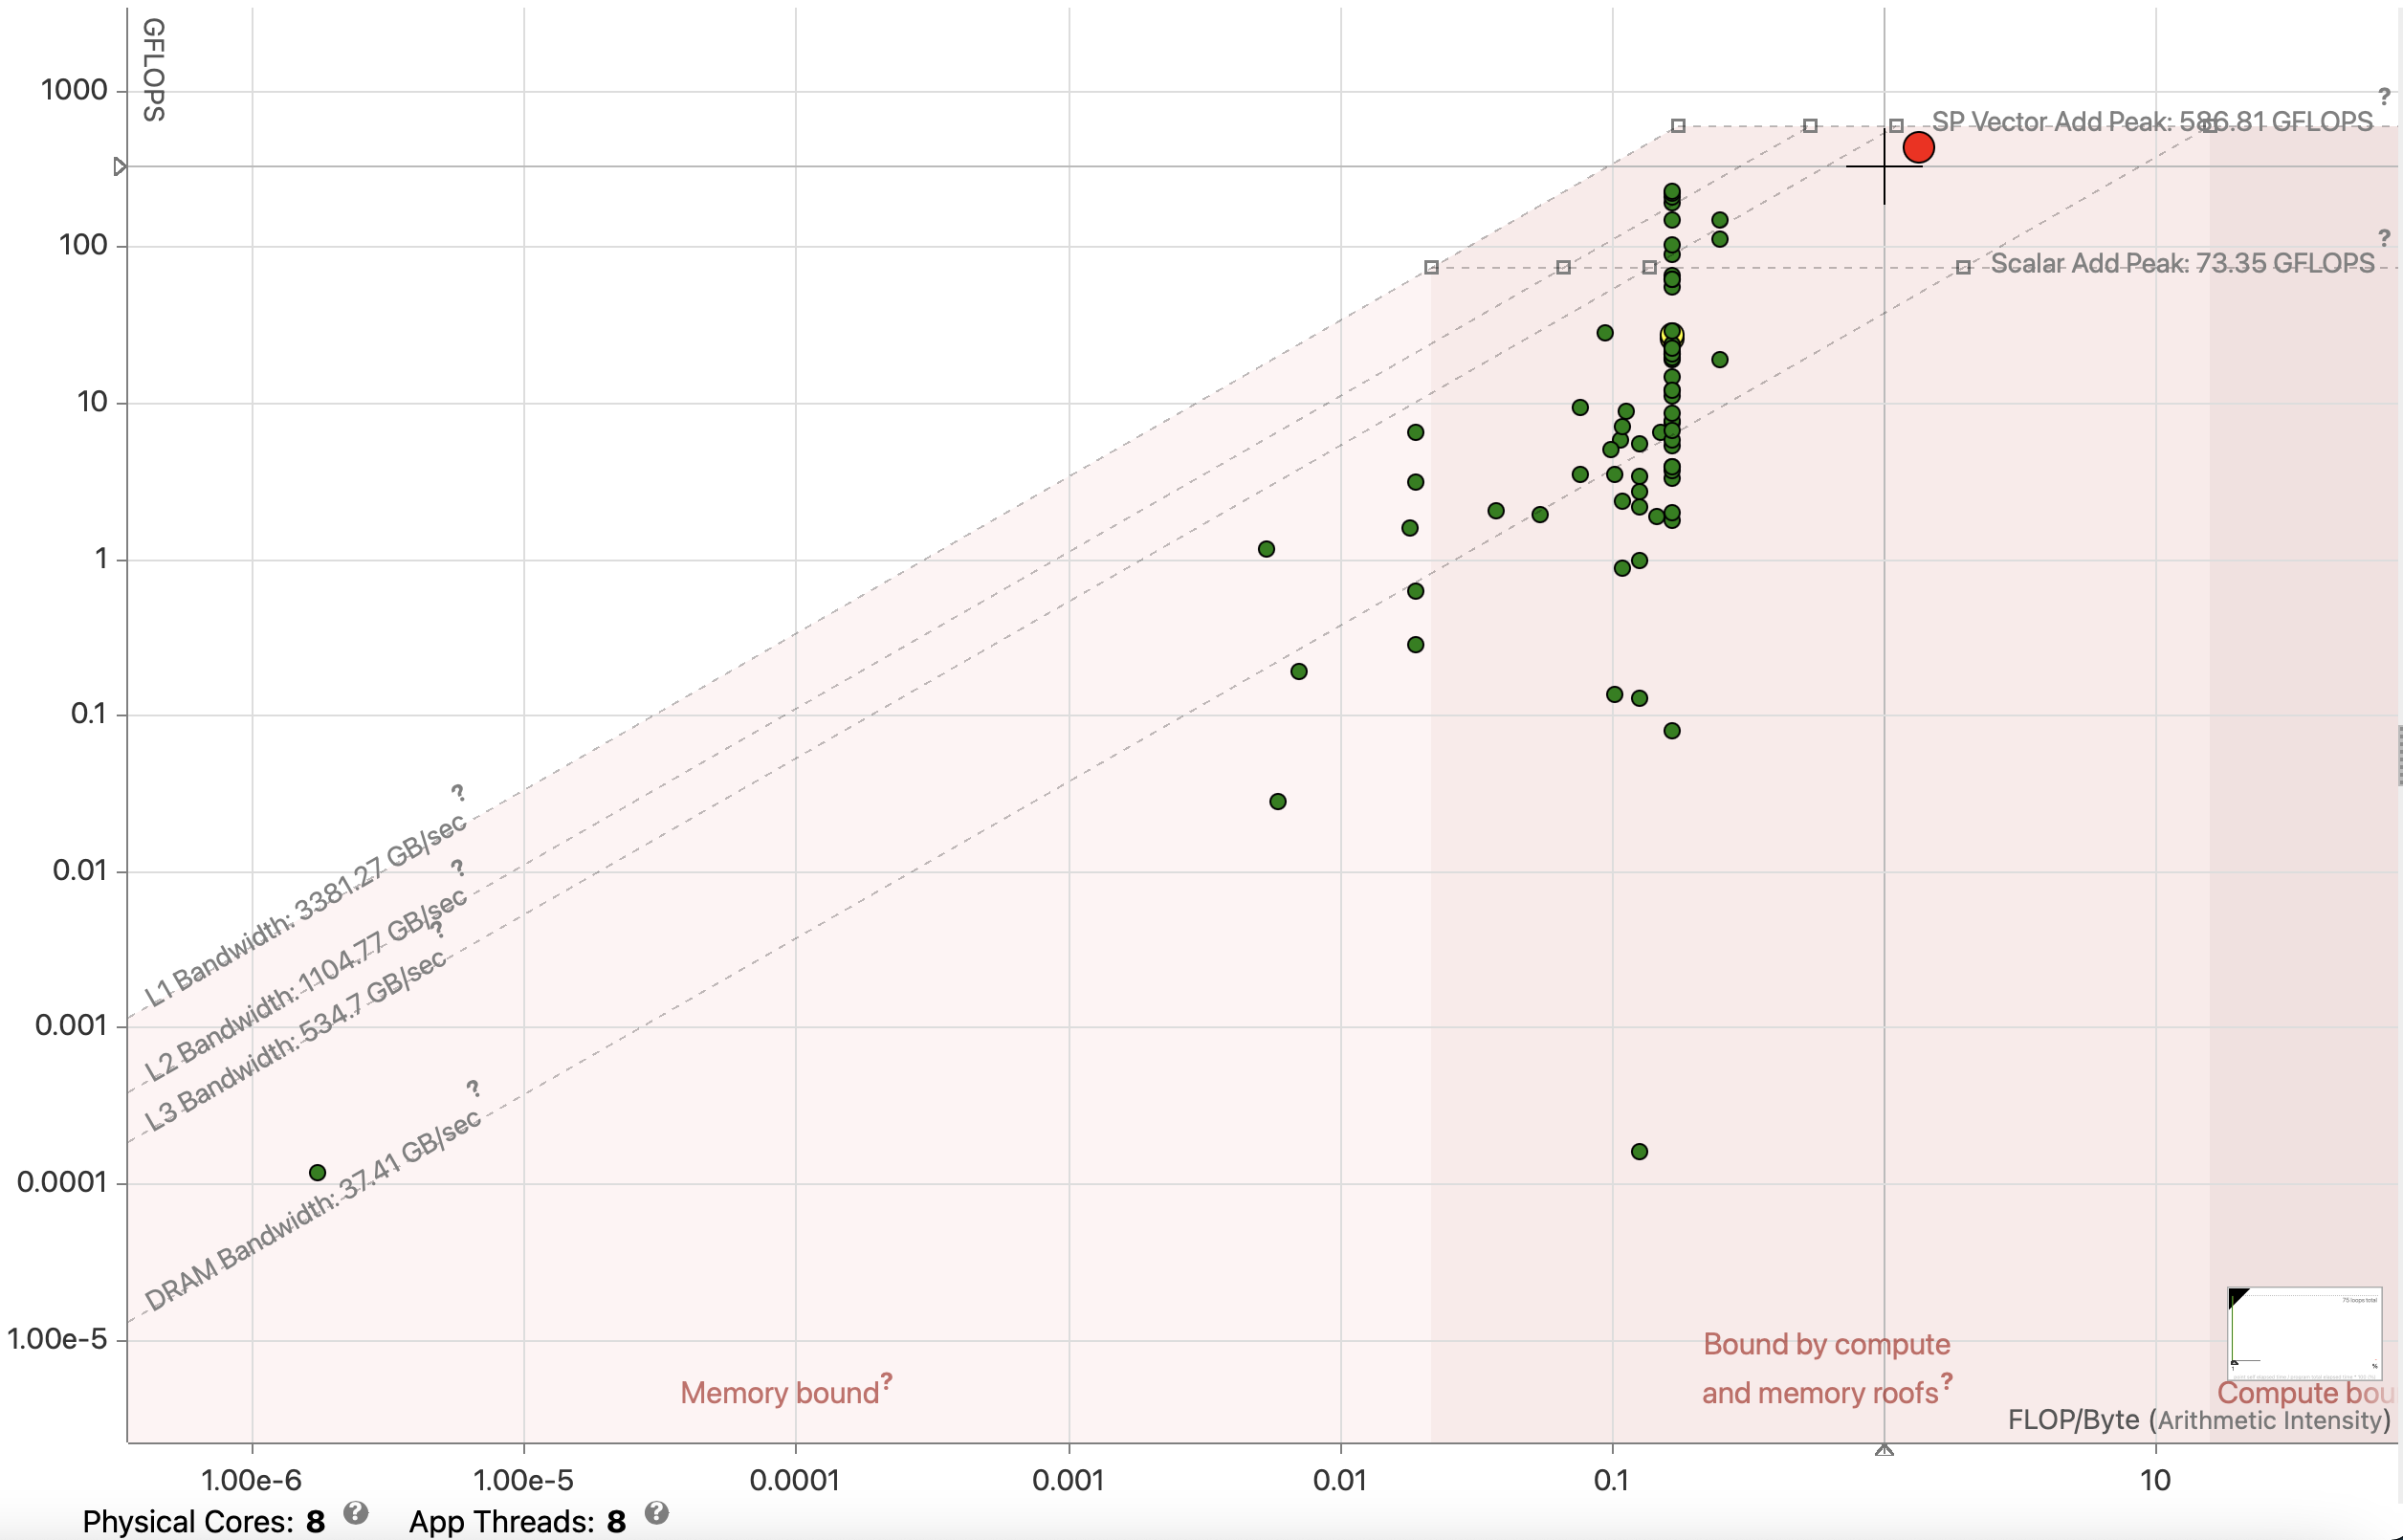
\includegraphics[scale=0.20, trim=0 0 0 0,clip]{content/figures/roofline_coffee_lake.png}}
\caption{Xeon E-2278G (Coffee Lake) roofline for max-plus}
\label{fig:roof_line_coffee_lake}
\end{figure}


{\textbf{Broadwell Roofline:}} Figure~\ref{fig:roof_line_broad_well} presents the Broadwell roofline model. From this roof line model, we observe that the attainable max-plus machine peak of Broadwell is around 165 GFLOPS, which is $85\%$ of the theoretical machine peak (192 GFLOPS) with the processor running at maximum frequency.

\begin{figure}[htbp]
\centerline{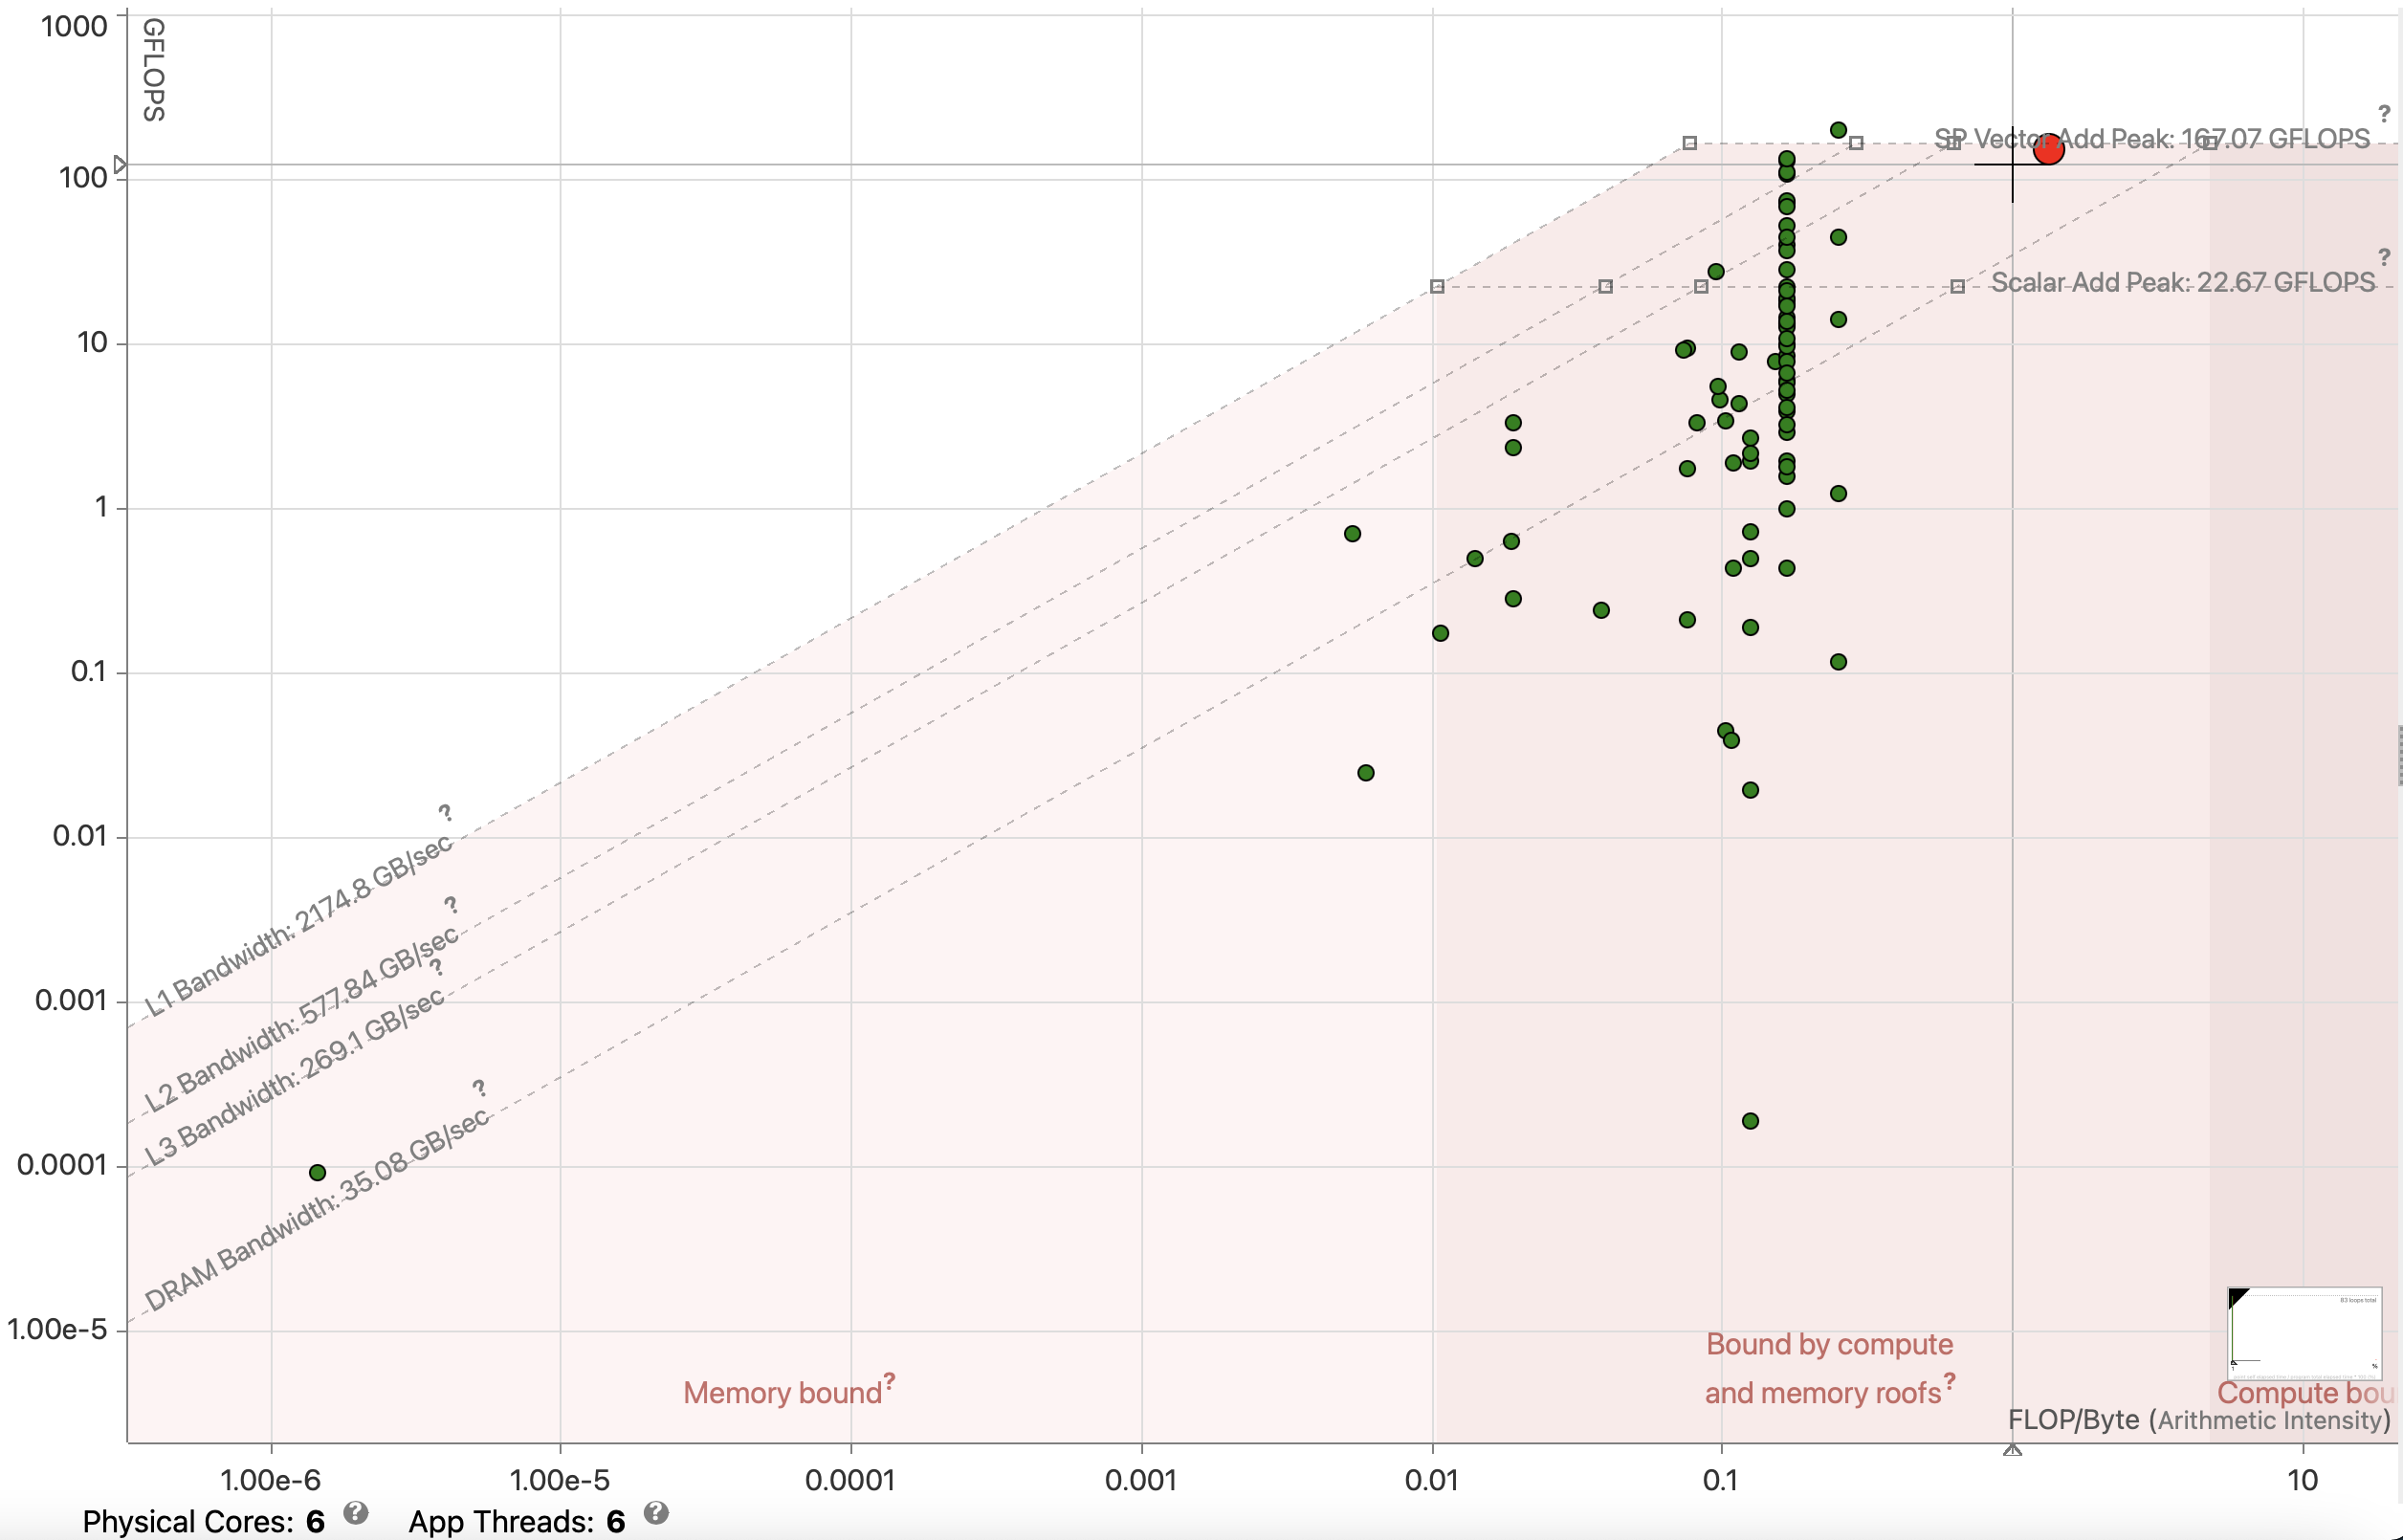
\includegraphics[scale=0.20, trim=0 0 0 0,clip]{content/figures/roofline_broadwell.png}}
\caption{Xeon E5 1650v4 (Broadwell) roofline for max-plus}
\label{fig:roof_line_broad_well}
\end{figure}


\subsubsection{Tile Parameter Exploration}
We use three levels of tiling (Fig~\ref{fig:bpmax_full_tiling}) in our optimization. The size of the first-level tile depends on the length of the second input sequence($N$), which is a program parameter. That leaves us to explore second and third-level tiling parameters. We have implemented a micro-kernel that performs matrix-max plus operation on two square matrices of size ($N \times N$) to explore the best register tile and mono-parametric tile parameter. We choose square matrices $(N = 2800)$ such that the footprint exceeds the L3 cache. Figure~\ref{fig:register_tile_performance_comparison} compares performance between different register tiles on Coffee Lake. We tile the three outer loops with a mono-parametric tile size of $192$. Then, we register-tile each patch. The register-tile kernel assumes that the data is accessed sequentially. All the results shown here include the packing operation of these patches.
\begin{figure}[htbp]
    \centering
    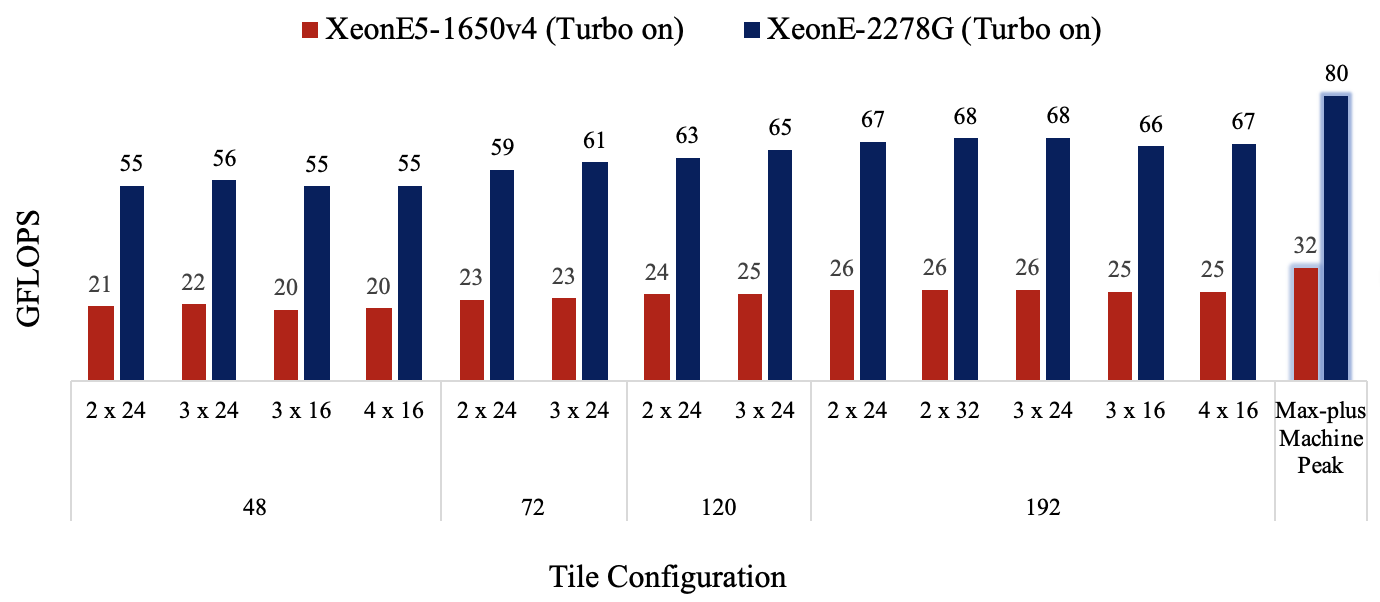
\includegraphics[scale=0.37, trim=4 4 4 4,clip]{content/figures/max_plus_register_tile_performance_new.png}
   \caption{Register-Tiled Max-plus Performance}
\label{fig:register_tile_performance_comparison}
\end{figure}
We notice that the register-tile $3 \times 24$ performs the best which matches our theoretical register allocation strategy. 
To explore second-level tile size, we fixed the register tile parameters and vary the second-level tile size [48, 72, 120, 192]. We find that the second-level tile size of 48 performs better than the others for double max-plus and BPMax when the register-tile size is $3 \times 24$. When $N_{tile}=48$, all the inputs and outputs of the register-tiled kernel fit in the $L_{1}$. So, we use $N_{tile}=48$ and the register-tile dimension of $3 \times 24$ for the rest of our experiments.



\subsection{Double Max-plus Performance Improvement}
\subsubsection{Single Core Performance}
Figure~\ref{fig:st_performance_analysis_double_max_plus} presents the performance of the double max-plus on single thread of Xeon E5-1650v4 (Broadwell) and Xeon E-2278G (Coffee Lake). We compare the performance between the best optimized previous version ~\cite{Mondal2021} and the current version with the diagonal schedule.
\begin{figure}[htbp]
\centerline{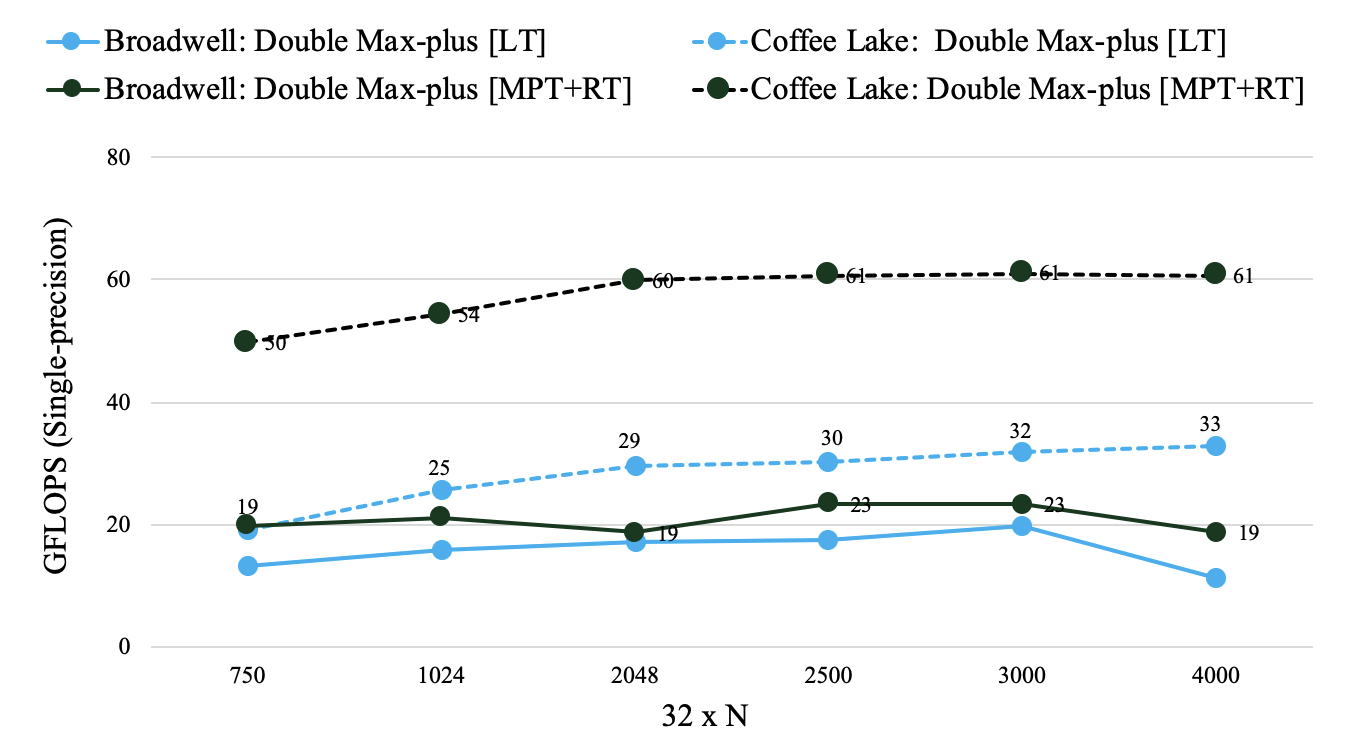
\includegraphics[scale=0.38, trim=5 5 5 5,clip]{content/figures/dpm_single_core_new.png}}
\caption{Double Max-plus Single Core Performance}
\label{fig:st_performance_analysis_double_max_plus}
\end{figure}
Figure~\ref{fig:st_performance_analysis_double_max_plus} shows the performance of the double max-plus computation with these two versions of the code, when $M$ is fixed to $32$ and $N$ is varied between $750$ to $4000$. We have not presented the base version since it only attains a tiny fractional GFLOPS performance. The previous best-optimized version of the program highlighted in sky-blue reaches about $50\%$ of the roofline machine peak on both Broadwell (dotted blue line) and Coffee Lake (dotted dark-green line), whereas the current best-optimized version attains over $90\%$ and $80\%$ of the max-plus roofline machine peak on Broadwell (dark-green continuous line) and Coffee Lake (dark-green dotted line), respectively. Both versions of the program performed poorly on Broadwell when $N$ was larger than $3000$. It is due to the $F$-Table memory footprint becoming close to Broadwell's DRAM capacity (16 GB) when $M=32$, $N=4000$, triggering swapping (disk-access) that reduces CPU resource utilization. We do not see this behavior on Coffee Lake.


\subsubsection{Multi-Core Performance Comparison}
For our experiments on multi-core, we choose three different values of $M$ ($16$, $25$, $32$) and five different values of $N$ ($750$, $1024$, $2048$, $2500$, $3000$) to measure the double max-plus performance for each combination of $M$ and $N$. Figure~\ref{fig:peroformance_analysis_double_max_plus} and Figure~\ref{fig:double_max_plus_speed_up} show the performance and speedup comparisons of double max-plus between the base schedule, previously optimized best version ([LT]), and current best-optimized version ( [MPT+RT]) with eight threads on Coffee Lake. The performance of the original code is about 1 GFLOPS, highlighted in dark red.
\begin{figure}[htbp]
\centerline{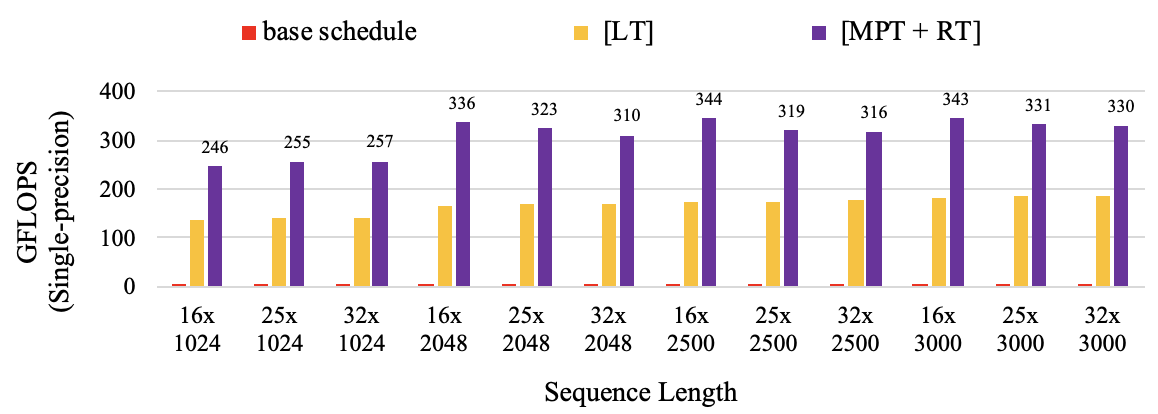
\includegraphics[scale=0.42, trim=5 5 5 5,clip]{content/figures/dpm_performance_new.png}}
\caption{Double Max-plus Performance, Coffee Lake }
\label{fig:peroformance_analysis_double_max_plus}
\end{figure}
\begin{figure}[htbp]
\centerline{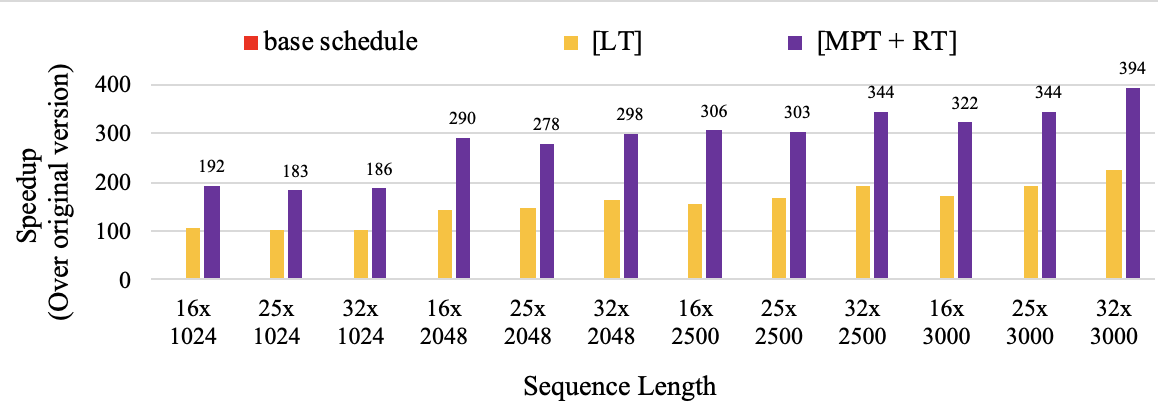
\includegraphics[scale=0.42, trim=5 5 5 5,clip]{content/figures/dpm_speedup_new.png}}
\caption{Double Max-plus Speedup, Coffee Lake}
\label{fig:double_max_plus_speed_up}
\end{figure}
The yellow color represents the performance corresponding to the [LT]. It attains a maximum performance of $187$ GFLOPS (32\% of the roofline machine peak) on Coffee Lake. The best [MPT+RT] version, represented by the purple color, reaches a peak performance of $344$ GFLOPS which is 58\% of the roofline machine peak. These correspond to a speed up of $223\times$ and $394\times$  over the implementation available in the original BPMax program.




\subsection{BPMax Performance Improvement}
We have chosen input parameters similar to Double max-plus to measure the BPMax performance.

\subsubsection{Single-Core Performance}
Figure~\ref{fig:st_performance_analysis_bpmax} shows the single core performance of the best BPMax version, \textbf{[MPT+RT]:v3} with $M=32$ and $N$ varying between ($750$, $1024$, $2048$, $2500$, $3000$, $4000$). We attain about 80\% and 85\% of the roofline max-plus machine peak on Coffee Lake and Broadwell, respectively.
\begin{figure}[htbp]
\centerline{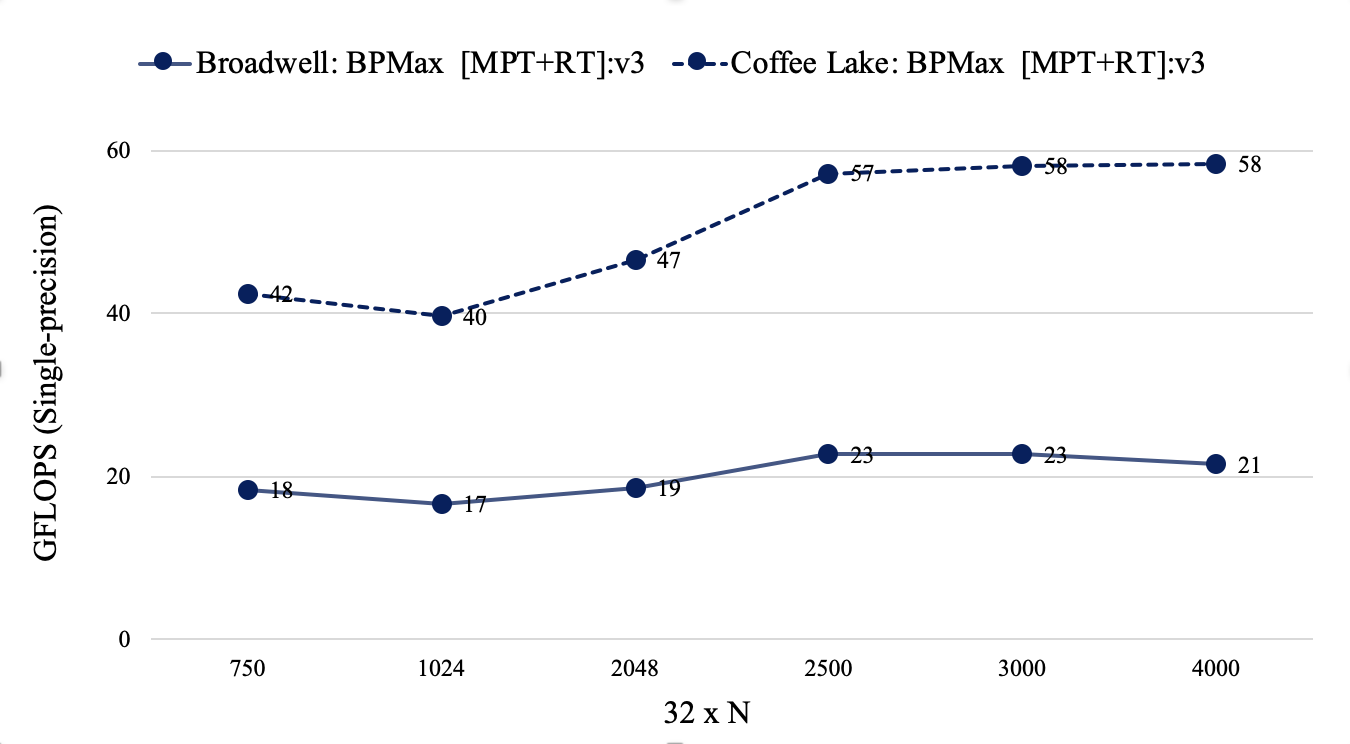
\includegraphics[scale=0.38, trim=5 5 5 5,clip]{content/figures/bpmax_single_core_new.png}}
\caption{BPMax Single Core Performance}
\label{fig:st_performance_analysis_bpmax}
\end{figure}

\subsubsection{Multi-Core Performance}

\begin{figure*}[htbp]
\centerline{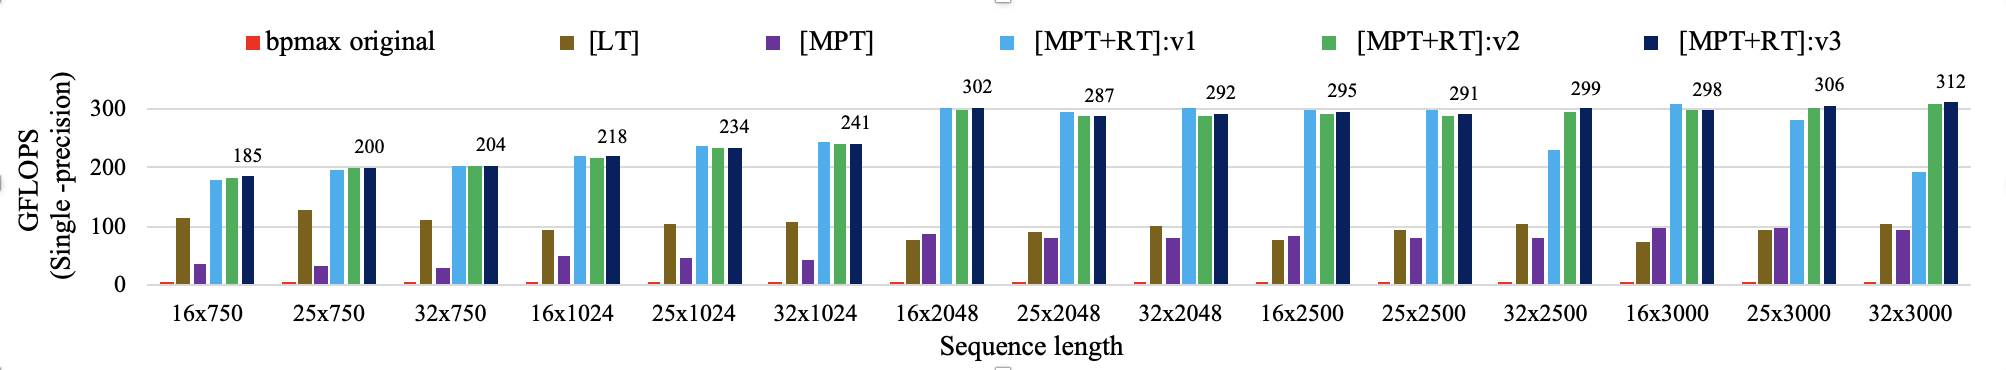
\includegraphics[width=\textwidth,scale=1.00, trim=5 5 5 5,clip]{content/figures/bpm_performance_new_tile.png}} 
\caption{BPMax performance comparison on Coffee Lake}
\label{fig:bpm_performance}
\end{figure*}

\begin{figure*}[htbp]
\centerline{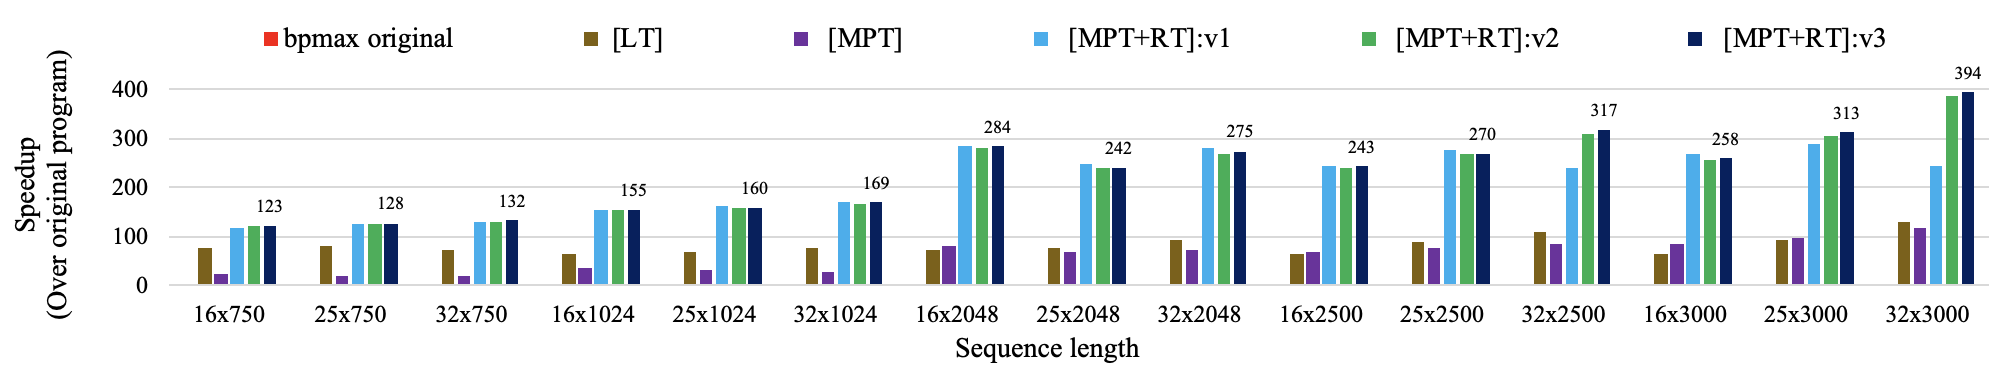
\includegraphics[width=\textwidth,scale=1.00, trim=5 5 5 5,clip]{content/figures/bpm_speed_up_new_tile.png}} 
\caption{BPMax speedup comparison on Coffee Lake}
\label{fig:bpm_speed_up}
\end{figure*}
Figure~\ref{fig:bpm_performance} and ~\ref{fig:bpm_speed_up} show the performance improvements and speedup of various versions of BPMax program on Coffee Lake with $8$ threads. We use the original implementation (BPMax original) as the reference highlighted in red. 
The performance and speedup with the best optimized previous version \cite{Mondal2021} ([LT]) is highlighted in brown. [LT] earlier achieved  $100\times$ speedup for longer sequence lengths. The last four data points use different versions of the current work.

The first data point [MPT] with our new implementation is highlighted in purple, which does not employ the register tiling but uses mono-parametric tiles for the second-level tile. It employs similar program transformations like all the versions of the [MPT] with register tiling to improve data locality for each tile. We observe that a mono-parametric tile size of 192 works better across all the inputs. [MPT] shows no performance improvement over [LT] because the best tile size was not long enough for effective vectorization.

We have experimented with three types of data-transformation techniques with our register-tiled code. \textbf{[MPT+RT]:v1} performs best when the memory footprint is low. As the memory footprint increases, it performs poorly. There is no significant differences between the \textbf{[MPT+RT]:v2} and \textbf{[MPT+RT]:v3}. However, the \textbf{[MPT+RT]:v3} performs consistently well across all the inputs. Figure~\ref{fig:bpm_performance} and~\ref{fig:bpm_speed_up} show the performance and speed up achieved by the \textbf{[MPT+RT]:v3}. It attains a peak performance of $53\%$ of the roofline machine peak on Coffee Lake, about $400\times$ faster than the base program. Figure~\ref{fig:roof_line_coffee_lake} shows the CPU usage of different parts of the BPmax program. We observe that $72\%$ of the program's execution time (139s/187s) is spent in the register-tiled kernel, which achieved $82\%$ of the roofline peak. The remaining $30\%$ of the program spent significant time in vectorized code and memory initialization. However, it is important to note that additional work is done when a mono-parametric tile is filled with max-plus identity values corresponding to the triangular tiles from the edge of the inner triangle. These additional computations over the identity elements are excluded from the GFLOPS computation reported in the figures. Our polyhedral compilation scripts and source codes are available in the GitHub repository\footnote{https://github.com/chiranjeb/BPMaxCPU}.



\section{Conclusion}\label{sec:future_directions}
In this work, we have demonstrated the optimization process of a complete RRI program using polyhedral code generation tool. We have explored different schedules, memory maps, and tiling transformations for our optimization work using the polyhedral code generator -  \alphaz\ .

We have explored multi-level tiling in our optimization work. We observe that a register-tiled kernel was easier to integrate when the program was transformed using mono-parametric tiling. Also, mono-parametric tiling enabled us to tile the nearly tile-able OSP-like inner-reductions ($R^{1}$ and $R^{2}$). We achieved more than $50\%$ of the roofline machine peak and improved the performance of the entire BPMax program by $400\times$. $70\%$ of this work got done by the register-tiled loop. Analysis from Intel Advisor shows that this loop attained $80\%$ of the roofline machine peak. In the future, it will be interesting to understand if there are further optimization opportunities like additional memory transformation to get close to the roofline machine peak.

We observed that double max-plus operation on single-core attained $80\%$ of the roofline machine peak. But, performance dropped to $53\%$ of the roofline machine peak with eight threads. So, finding opportunities to mitigate the scheduling and communication latency between the threads will be interesting. Our optimization work focused on the Intel platform. However, a future direction will be implementing the register-tiled kernel for a different processor architecture like AMD and comparing the performance improvement. In the long term, it can also be beneficial to distribute the computation over a cluster using MPI (Message Passing Interface) program to take advantage of another level of parallelism. All these transformations remain a challenge for \alphaz\ today. So, we also envision future work on \alphaz\ to allow these advanced transformations.

%Finally, we expect similar polyhedral transformations to be easily applied to more complex RRI algorithms like BPPart and piRNA using \alphaz\ to generate optimized code and achieve significant speedup.





%\subsection{Subsection Heading Here}
%Subsection text here.

% needed in second column of first page if using \IEEEpubid
%\IEEEpubidadjcol

%\subsubsection{Subsubsection Heading Here}
%Subsubsection text here.


% An example of a floating figure using the graphicx package.
% Note that \label must occur AFTER (or within) \caption.
% For figures, \caption should occur after the \includegraphics.
% Note that IEEEtran v1.7 and later has special internal code that
% is designed to preserve the operation of \label within \caption
% even when the captionsoff option is in effect. However, because
% of issues like this, it may be the safest practice to put all your
% \label just after \caption rather than within \caption{}.
%
% Reminder: the "draftcls" or "draftclsnofoot", not "draft", class
% option should be used if it is desired that the figures are to be
% displayed while in draft mode.
%
%\begin{figure}[!t]
%\centering
%\includegraphics[width=2.5in]{myfigure}
% where an .eps filename suffix will be assumed under latex, 
% and a .pdf suffix will be assumed for pdflatex; or what has been declared
% via \DeclareGraphicsExtensions.
%\caption{Simulation results for the network.}
%\label{fig_sim}
%\end{figure}

% Note that the IEEE typically puts floats only at the top, even when this
% results in a large percentage of a column being occupied by floats.
% However, the Computer Society has been known to put floats at the bottom.


% An example of a double column floating figure using two subfigures.
% (The subfig.sty package must be loaded for this to work.)
% The subfigure \label commands are set within each subfloat command,
% and the \label for the overall figure must come after \caption.
% \hfil is used as a separator to get equal spacing.
% Watch out that the combined width of all the subfigures on a 
% line do not exceed the text width or a line break will occur.
%
%\begin{figure*}[!t]
%\centering
%\subfloat[Case I]{\includegraphics[width=2.5in]{box}%
%\label{fig_first_case}}
%\hfil
%\subfloat[Case II]{\includegraphics[width=2.5in]{box}%
%\label{fig_second_case}}
%\caption{Simulation results for the network.}
%\label{fig_sim}
%\end{figure*}
%
% Note that often IEEE papers with subfigures do not employ subfigure
% captions (using the optional argument to \subfloat[]), but instead will
% reference/describe all of them (a), (b), etc., within the main caption.
% Be aware that for subfig.sty to generate the (a), (b), etc., subfigure
% labels, the optional argument to \subfloat must be present. If a
% subcaption is not desired, just leave its contents blank,
% e.g., \subfloat[].


% An example of a floating table. Note that, for IEEE style tables, the
% \caption command should come BEFORE the table and, given that table
% captions serve much like titles, are usually capitalized except for words
% such as a, an, and, as, at, but, by, for, in, nor, of, on, or, the, to
% and up, which are usually not capitalized unless they are the first or
% last word of the caption. Table text will default to \footnotesize as
% the IEEE normally uses this smaller font for tables.
% The \label must come after \caption as always.
%
%\begin{table}[!t]
%% increase table row spacing, adjust to taste
%\renewcommand{\arraystretch}{1.3}
% if using array.sty, it might be a good idea to tweak the value of
% \extrarowheight as needed to properly center the text within the cells
%\caption{An Example of a Table}
%\label{table_example}
%\centering
%% Some packages, such as MDW tools, offer better commands for making tables
%% than the plain LaTeX2e tabular which is used here.
%\begin{tabular}{|c||c|}
%\hline
%One & Two\\
%\hline
%Three & Four\\
%\hline
%\end{tabular}
%\end{table}


% Note that the IEEE does not put floats in the very first column
% - or typically anywhere on the first page for that matter. Also,
% in-text middle ("here") positioning is typically not used, but it
% is allowed and encouraged for Computer Society conferences (but
% not Computer Society journals). Most IEEE journals/conferences use
% top floats exclusively. 
% Note that, LaTeX2e, unlike IEEE journals/conferences, places
% footnotes above bottom floats. This can be corrected via the
% \fnbelowfloat command of the stfloats package.




%\section{Conclusion}
%The conclusion goes here.





% if have a single appendix:
%\appendix[Proof of the Zonklar Equations]
% or
%\appendix  % for no appendix heading
% do not use \section anymore after \appendix, only \section*
% is possibly needed

% use appendices with more than one appendix
% then use \section to start each appendix
% you must declare a \section before using any
% \subsection or using \label (\appendices by itself
% starts a section numbered zero.)
%


%\appendices
%\section{Proof of the First Zonklar Equation}
%Appendix one text goes here.

% you can choose not to have a title for an appendix
% if you want by leaving the argument blank
%\section{}
%Appendix two text goes here.


% use section* for acknowledgment
%\ifCLASSOPTIONcompsoc
  % The Computer Society usually uses the plural form
%  \section*{Acknowledgments}
%\else
  % regular IEEE prefers the singular form
%  \section*{Acknowledgment}
%\fi


%The authors would like to thank...


% Can use something like this to put references on a page
% by themselves when using endfloat and the captionsoff option.
\ifCLASSOPTIONcaptionsoff
  \newpage
\fi



% trigger a \newpage just before the given reference
% number - used to balance the columns on the last page
% adjust value as needed - may need to be readjusted if
% the document is modified later
%\IEEEtriggeratref{8}
% The "triggered" command can be changed if desired:
%\IEEEtriggercmd{\enlargethispage{-5in}}

% references section

% can use a bibliography generated by BibTeX as a .bbl file
% BibTeX documentation can be easily obtained at:
% http://mirror.ctan.org/biblio/bibtex/contrib/doc/
% The IEEEtran BibTeX style support page is at:
% http://www.michaelshell.org/tex/ieeetran/bibtex/

\bibliographystyle{IEEEtran}
% argument is your BibTeX string definitions and bibliography database(s)
\bibliography{IEEEabrv,content/bpmax}
%
% <OR> manually copy in the resultant .bbl file
% set second argument of \begin to the number of references
% (used to reserve space for the reference number labels box)

%\bibliography{sections/sample}

%\begin{thebibliography}{1}

%\bibitem{IEEEhowto:kopka}
%H.~Kopka and P.~W. Daly, \emph{A Guide to \LaTeX}, 3rd~ed.\hskip 1em plus
%  0.5em minus 0.4em\relax Harlow, England: Addison-Wesley, 1999.

%\end{thebibliography}

% biography section
% 
% If you have an EPS/PDF photo (graphicx package needed) extra braces are
% needed around the contents of the optional argument to biography to prevent
% the LaTeX parser from getting confused when it sees the complicated
% \includegraphics command within an optional argument. (You could create
% your own custom macro containing the \includegraphics command to make things
% simpler here.)
%\begin{IEEEbiography}[{\includegraphics[width=1in,height=1.25in,clip,keepaspectratio]{mshell}}]{Michael Shell}
% or if you just want to reserve a space for a photo:

%\begin{IEEEbiography}{Michael Shell}
%Biography text here.
%\end{IEEEbiography}

% if you will not have a photo at all:
%\begin{IEEEbiographynophoto}{John Doe}
%Biography text here.
%\end{IEEEbiographynophoto}

% insert where needed to balance the two columns on the last page with
% biographies
%\newpage

%\begin{IEEEbiographynophoto}{Jane Doe}
%Biography text here.
%\end{IEEEbiographynophoto}

% You can push biographies down or up by placing
% a \vfill before or after them. The appropriate
% use of \vfill depends on what kind of text is
% on the last page and whether or not the columns
% are being equalized.

%\vfill

% Can be used to pull up biographies so that the bottom of the last one
% is flush with the other column.
%\enlargethispage{-5in}

\vspace{4mm}
\begin{wrapfigure}{l}{0.10\textwidth}
    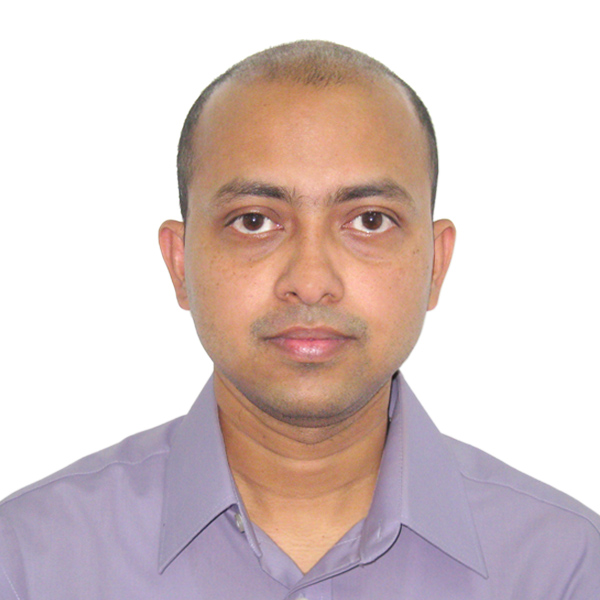
\includegraphics[width=0.10\textwidth]{content/figures/chiranjeb.JPG}
\end{wrapfigure}
Chiranjeb Mondal received his Bachelor of Engineering in Computer Science and Engineering from the National Institute of Technology, Durgapur, India, in 2004 and his Master of Science in Computer Science from Colorado State University, USA, in 2020. Currently, he is a Ph.D. student working on performance improvement using polyhedral compilation.


\vspace{1mm}
\begin{wrapfigure}{l}{0.10\textwidth}
    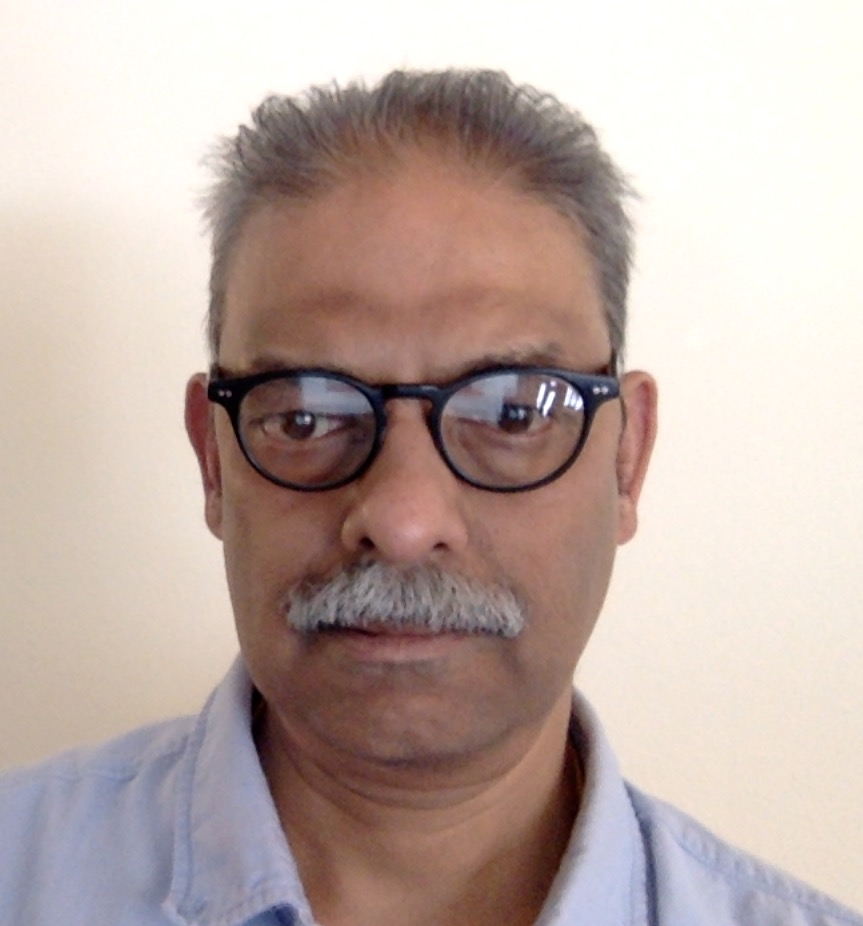
\includegraphics[width=0.10\textwidth]{content/figures/sanjay.png}
\end{wrapfigure}
Sanjay Rajopadhye received his Bachelor of Technology (honours) in Electrical Engineering from the Indian Institute of Technology, Kharagpur, in 1980, and the Ph.D. in Computer Science from the University of Utah in 1986. He held academic positions at the University of Oregon, Oregon State University, and IRISA, Rennes. He is currently a professor in the Computer Science (CS) and in the Electrical and Computer Engineering (ECE) departments at Colorado State University. He is one of the inventors of the polyhedral model.  His Ph.D. dissertation made three key contributions to the foundations of the polyhedral model: scheduling, locality, and closure.

\end{document}


